\documentclass[letterpaper,final,12pt,reqno]{amsart}

\usepackage[total={6.3in,9.2in},top=1.1in,left=1.1in]{geometry}

\usepackage{times,bm,bbm,empheq,fancyvrb,graphicx}
\usepackage[dvipsnames]{xcolor}
\usepackage{longtable}
\usepackage{booktabs}

\usepackage{tikz}
\usetikzlibrary{decorations.pathreplacing}

\usepackage[kw]{pseudo}
\pseudoset{left-margin=15mm,topsep=5mm,idfont=\texttt}

% hyperref should be the last package we load
\usepackage[pdftex,
colorlinks=true,
plainpages=false, % only if colorlinks=true
linkcolor=blue,   % ...
citecolor=Red,    % ...
urlcolor=black    % ...
]{hyperref}

\renewcommand{\baselinestretch}{1.05}

\newtheoremstyle{claim}% name
  {5pt}% space above
  {5pt}% space below
  {\itshape}% body font
  {}% indent amount
  {\itshape}% theorem head font
  {.}% punctuation after theorem head
  {.5em}% space after theorem head
  {\thmname{#1}\thmnumber{ #2}\thmnote{ (#3)}}% theorem head spec
\theoremstyle{claim}
\newtheorem{theorem}{Theorem}
\newtheorem{lemma}{Lemma}

\newcommand{\eps}{\epsilon}
\newcommand{\RR}{\mathbb{R}}

\newcommand{\grad}{\nabla}
\newcommand{\Div}{\nabla\cdot}
\newcommand{\trace}{\operatorname{tr}}

\newcommand{\hbn}{\hat{\mathbf{n}}}

\newcommand{\bb}{\mathbf{b}}
\newcommand{\be}{\mathbf{e}}
\newcommand{\bbf}{\mathbf{f}}
\newcommand{\bg}{\mathbf{g}}
\newcommand{\bn}{\mathbf{n}}
\newcommand{\br}{\mathbf{r}}
\newcommand{\bu}{\mathbf{u}}
\newcommand{\bv}{\mathbf{v}}
\newcommand{\bw}{\mathbf{w}}
\newcommand{\bx}{\mathbf{x}}

\newcommand{\bF}{\mathbf{F}}
\newcommand{\bV}{\mathbf{V}}
\newcommand{\bX}{\mathbf{X}}

\newcommand{\bxi}{\bm{\xi}}

\newcommand{\bzero}{\bm{0}}

\newcommand{\rhoi}{\rho_{\text{i}}}

\newcommand{\ip}[2]{\left<#1,#2\right>}

\newcommand{\mR}{R^{\bm{\oplus}}}

% numbering
\setcounter{tocdepth}{3}
\makeatletter
\def\l@subsection{\@tocline{2}{0pt}{4pc}{5pc}{}}
\makeatother

\numberwithin{equation}{section}
\numberwithin{figure}{section}
\numberwithin{table}{section}
\numberwithin{theorem}{section}


\begin{document}
\title[Geometric multigrid for glacier modeling]{Geometric multigrid for glacier modeling: \\ New techniques and concepts}

\author{Ed Bueler}

\begin{abstract} FIXME: two principles in introduction: mass conservation complementarity, solver optimality.  four examples in sections \ref{sec:subspace}--\ref{sec:stokes}: poisson equation from subspace decomp point of view, obstacle problem by subset decomposition, monotone multigrid for implicitly-evolving SIA geometry, Schur-complement and Vanka Newton-multigrid for fixed-geometry Glen-Stokes
\end{abstract}

\maketitle

\tableofcontents

\thispagestyle{empty}
\bigskip

\section{Introduction} \label{sec:intro}

The construction of effective numerical glacier and ice sheet models is challenging for two fundamental reasons.  First is the complexity of the equations and boundary conditions.  Indeed, the physics of glaciers is nonlinear, nontrivially-coupled, and subject to imperfectly-understood boundary processes, such as at contact with ocean water.  The coupling is critical in the sense that mass, momentum, and energy conservation interact in ways which are relevant to glaciological modeling goals, such as when basal sliding, and thus ice velocity, is only determined though a simultaneous momentum and energy solution.  Second, the geometry of glaciers and ice sheets is complex, and in particular the fastest-flowing parts of ice sheets are often located at the geometrically-nontrivial lateral boundary where fjord-like bed geometry is also common.  Numerical models therefore need to perform expensive fine-mesh calculations, so as to accomodate the complicated, changing boundary geometry, while solving relatively-complicated multiphysics equations.

On the other hand, since the 1980s researchers in numerial methods have developed multigrid methods to solve partial differential equations like those which describe the ice fluid in glaciers.   For simpler problems like scalar elliptic equations and the linear Stokes system, especially on domains which have a simpler geometry, these methods are now in routine use \cite{Briggsetal2000,Bueler2021,Trottenbergetal2001}.

FIXME Accessible introductions to FE methods are in \cite{Bueler2021,Elmanetal2014,Johnson2009}.  Closest to our view in section \ref{sec:subspace} is \cite[Chapter V]{Braess2007}

FIXME cite for multigrid on classical obstacle \cite{BrandtCryer1983,Bueler2021,GraeserKornhuber2009}


\section{Subspace decomposition, and geometric multigrid} \label{sec:subspace}

\subsection*{Finite elements for a Poisson model problem}  In this section we will consider how to solve a simple differential equation, namely a linear Poisson-like problem
\begin{equation}
- \big(\alpha(x)\,u'(x)\big)' = f(x) \quad \text{on} \quad 0 \le x \le 1, \label{eq:poisson}
\end{equation}
with Dirichlet boundary conditions $u(0)=u(1)=0$, using a finite element discretization and a multigrid method.  The functions $\alpha(x)$ and $f(x)$ are the given data here, assumed sufficiently well-behaved for the computations which follow, and we assume $\alpha(x)$ is bounded and positive so the problem is elliptic \cite{Evans2010}: $0 < c_1 \le \alpha(x) \le c_2$.  Over the course of the next three sections, this simple problem will evolve into a realistic model for glacier geometry.

Our numerical approximation of \eqref{eq:poisson} uses a mesh of $m$ interior \emph{nodes} (points) $x_p$ on $(0,1)$.  The $m+1$ intervals between the nodes are the \emph{elements}.  The numerical solution $u^h(x)$ is then a linear combination of the piecewise-linear \emph{hat functions} $\psi_p(x)$, shown in Figure \ref{fig:finehats}, one for each interior node:
\begin{equation}
u^h(x) = \sum_{p=1}^m u_p \psi_p(x). \label{eq:trialsolution}
\end{equation}
Each hat function $\psi_p(x)$ is continuous on $[0,1]$, linear on each element, and satisfies $\psi_p(x_q) = \delta_{pq}$.  The set $\{\psi_p(x)\}_{p=1}^m$ is a \emph{nodal basis} of the space $\mathcal{V}^h$ of continuous, piecewise-linear functions; the coefficients equal the function values: $u_p=u^h(x_p)$.  Note that the derivative of $u^h(x)$ is well-defined on the elements, thus almost everywhere, but not at the nodes.  In a computer program the coefficients $u_p$ will be formed into a (column) vector $\bu=\{u_p\}$ in $\RR^m$.

\begin{figure}
\includegraphics[width=0.65\textwidth]{genfigs/finehats.pdf}
\caption{Hat functions $\psi_p(x)$ at interior points $x_p$ form a basis for a vector space $\mathcal{V}^h$ of piecewise-linear functions.}
\label{fig:finehats}
\end{figure}

As usual in numerical differential equations, we are interested in the fine-mesh limit where $m$ is large.  Previewing the glacier problems in upcoming sections, what is the need for a high-resolution mesh, i.e.~a large value of $m$ and small spacing between the nodes $x_p$?  For an ice sheet model, the need is obvious: a high-resolution mesh can capture realistically-bumpy bed topography and spatially-varying climatic mass-balance.  These fields roughly correspond in problem \eqref{eq:poisson} to variations in the coefficient function $\alpha(x)$ and the source function $f(x)$, respectively.  We will need the mesh to be \emph{fine}, i.e.~high-resolution, so as to capture the fine scales in these model input data.  In addition, as we start to address in section \ref{sec:obstacle}, a fine mesh will allow precise modeling of glacier extent and the location of glacier margins.

Our application of multigrid ideas to glacier problems will use finite element (FE) concepts, and therefore we must rephrase \eqref{eq:poisson} into \emph{weak form} using integrals.  (The original equation will be called the \emph{strong form}.)  To do this we suppose that the solution $u(x)$ comes from a vector space $\mathcal{H}$ of functions which have values of zero at $x=0$ and $x=1$, and are smooth enough to make sense of the form which follows.  While we will not over-use this mathematical language, in fact $\mathcal{H}=H_0^1[0,1]=W_0^{1,2}[0,1]$ is a Hilbert and Sobolev space \cite[for example]{Evans2010} consisting of functions with one square-integrable derivative.  Also, we assume $\alpha(x)$ is at least in $L^\infty[0,1]$ and $f(x)$ at least in $L^2[0,1]$.

The weak form arises by multiplying both sides of \eqref{eq:poisson} by a \emph{test function} from $\mathcal{H}$ and integrating by parts so that only first derivatives remain.  Denoting the test function as $v(x)$, integrating on $[0,1]$, and using $v(0)=v(1)=0$, we find
\begin{equation}
\int_0^1 \alpha(x) u'(x) v'(x)\,dx = \int_0^1 f(x) v(x)\, dx.  \label{eq:weakpoissonearly}
\end{equation}
We now write this equation more compactly as
\begin{equation}
  a(u,v) = \ip{f}{v}, \label{eq:weakpoisson}
\end{equation}
defining each side as in \eqref{eq:weakpoissonearly}; we seek $u$ in $\mathcal{H}$ so that \eqref{eq:weakpoisson} holds for all $v$ in $\mathcal{H}$.  The left side functional $a(u,v)$ is linear in each argument (\emph{bilinear}) while the right side defines a \emph{linear functional} $\ell[v] = \ip{f}{v}$ acting on $v$ in $\mathcal{H}$.  (The convenience of such abstract notation will become clear as we describe multilevel algorithms.)

Our FE method seeks a solution $u^h$ in $\mathcal{V}^h$ of the same, but now finite-dimensional, weak-form,
\begin{equation}
  a(u^h,v) = \ip{f}{v},  \label{eq:feweakpoisson}
\end{equation}
for all test functions $v$ in $\mathcal{V}^h$.  However, $\mathcal{V}^h$ is a subset of $\mathcal{H}$ so we can compare $u^h$ and $u$.  In fact, by subtracting \eqref{eq:feweakpoisson} from \eqref{eq:weakpoisson} we see that the \emph{numerical error} $u-u^h$ satisfies the simple equation $a(u-u^h,v)=0$ for all $v$ in $\mathcal{V}^h$.  That is, the numerical error is orthogonal, in the sense determined by $a(\cdot,\cdot)$, to the finite-dimensional subspace $\mathcal{V}^h$.  Standard FE arguments then show that the error goes to zero as $h$ goes to zero \cite{Braess2007,Elmanetal2014}.

One may substitute formula \eqref{eq:trialsolution} for $u^h$ into \eqref{eq:feweakpoisson} to derive a linear system
\begin{equation}
A \bu = \bbf, \label{eq:linearsystem}
\end{equation}
where $A$ is an $m\times m$ matrix and $\bbf$ is in $\RR^m$.  Each equation (row) in system \eqref{eq:linearsystem} is constructed by using a hat function as a test function; substitution of $v=\psi_p$ gives the $p$th equation.  The matrix $A$ has entries $a_{pq} = a(\psi_p,\psi_q)$, is symmetric, and is positive definite.  For the right side one defines entries $f_p = \ip{f}{\psi_p}$ to form the vector $\bbf = \{f_p\}$.  For the 1D problem here, only three values $a_{p,p-1}, a_{p,p}, a_{p,p+1}$ are nonzero in row $p$, so $A$ is tridiagonal.  (Writing these entries in detail, a worthy exercise, may remind the reader of finite difference approximations for the Laplacian.)

Depending on the form of $\alpha(x)$, the matrix entries
\begin{equation}
  a_{pq} = \int_0^1 \alpha(x) \psi_p'(x) \psi_q'(x)\,dx \label{eq:poissonentries}
\end{equation}
may be computed either exactly, or approximately by quadrature, and similar considerations apply to the values $f_p = \int_0^1 f(x) \psi_p(x)\,dx$.  The errors arising from doing these integrals by quadrature will have only a modest effect on the accuracy of the whole FE method \cite{Braess2007}.

The most straightforward way to solve assembled linear system \eqref{eq:linearsystem} would be via a ``direct'' method like Gaussian elimination.  In 2D and 3D problems, where the number of unknowns $m$ is large, such direct methods need much more that $O(m)$ operations to solve the system, while, as noted in the introduction, our applications demand optimal $O(m)$ solution methods, or nearly so.  Furthermore, excluding the current section, all of our problems will be nonlinear, thus no finite-time direct method will be available anyway.  Thus we will generally not assemble matrices, but instead construct rapidly-convergent iterations using easy-to-implement pointwise iterations and multiple mesh levels.

Our solution methods will be phrased in terms of ``residuals''.  Suppose $w$ in $\mathcal{V}^h$ is any estimate of the solution $u^h$ of \eqref{eq:feweakpoisson}.  We define the \emph{residual} of $w$ as a linear functional acting on $v$ in $\mathcal{V}^h$:
\begin{equation}
  F(w)[v] = a(w,v) - \ip{f}{v}.  \label{eq:residual}
\end{equation}
Finding $u^h$ is equivalent to making all components of its residual, i.e.~all values $F(w)[v]$ for $v$ in $\mathcal{V}^h$, zero:
\begin{equation}
  F(u^h)[v]=0 \qquad \text{ if and only if } \qquad a(u^h,v)=\ip{f}{v}. \label{eq:residualweakequivalence}
\end{equation}

Given $w$ which does not already solve \eqref{eq:feweakpoisson}, we will iteratively update it using simple operations which make residual components $F(w)[v]$ smaller.  Similarly to \eqref{eq:trialsolution}, we may represent $w$ using the basis of hat functions, i.e.~$w = \sum w_q \psi_q$ with $w_q = w(x_q)$, and then compute a component in this basis using the linearity of $a(\cdot,\cdot)$:
\begin{equation}
  F(w)[\psi_p] = \sum_{q=1}^{m} a(\psi_q,\psi_p) \,w(x_q) - \ip{f}{\psi_p}.  \label{eq:residualpoisson}
\end{equation}

The number of nonzero terms in sum \eqref{eq:residualpoisson} is equal to the number of hat functions $\psi_q$ whose support overlaps the support of $\psi_p$.  This number is at most three in the current 1D case, and for general 2D and 3D meshes it remains small if the elements do not have small angles \cite{Braess2007}.  Thus the computation of a component $F(w)[\psi_p]$ requires $O(1)$ work, so computing all components of a residual linear functional $F(w)$ requires $O(m)$ work.  This observation about the cost of evaluating a residual is foundational in all of our methods.

\subsection*{Coarse mesh levels and subspace decompositions}  From the above simple FE scheme we now take the first steps to build a \emph{multilevel} scheme.  Consider an enlarged set of hat functions:
    $$\underbrace{\psi_1(x),\dots,\psi_m(x)}_{\text{existing fine level}},\underbrace{\psi_{m+1}(x),\dots,\psi_M(x)}_{\text{\small coarser levels}}$$
For example, two coarser levels, derived from the fine level in Figure \ref{fig:finehats} by coarsening, are shown in Figure \ref{fig:coarsehats}.  The first coarsening (top) by-passes every other node on the fine mesh, and the next coarsening (bottom) does this again.

\begin{figure}
\includegraphics[width=0.55\textwidth]{genfigs/coarsehats.pdf}
\smallskip

\includegraphics[width=0.55\textwidth]{genfigs/coarsesthats.pdf}
\caption{Coarser levels are additional sets of hat functions which spread over a greater distance.}
\label{fig:coarsehats}
\end{figure}

On 2D and 3D meshes this manner of constructing coarse-mesh hats is less straightforward, and it is more common to start from a coarse mesh and refine level-by-level up to the finest.  In any case, our methods are not restricted to equally-spaced meshes, and models with a high-resolution structured mesh \cite[for example]{Bueler2016,Winkelmannetal2011} are among our target applications. We will return to these mesh-generation issues in section \ref{sec:sia}.

We need notation for the levels.  Suppose that the coarsest level is indexed as $j=0$ and the finest as $j=J$, and that the hat functions $\psi_p^j(x)$, for $p=1,\dots,m_j$, form the $j$th level.  The interior nodes $x_p^j$ use the same multilevel indexing scheme.  For example, Figures \ref{fig:finehats} and \ref{fig:coarsehats} show a three-level scheme ($J=2$) with $m_2=7$ fine-level, $m_1=3$ middle-level, and $m_0=1$ coarsest-level hat functions.  The original mesh has $m_2+1=8$ elements, divisible by four, so this three-level coarsening was allowed.  Note that the original fine level has now gained a superscript $J$; the original hats are $\psi_p^J(x)$ and the original nodes are $x_p^J$.

On each level the hat functions are linearly-independent and form a basis for a vector space:
\begin{equation}
  \mathcal{V}^j = \operatorname{span}\{\psi_1^j(x),\dots,\psi_{m_j}^j(x)\} \subset \mathcal{H}.  \label{eq:definevk}
\end{equation}
These spaces are nested, i.e.~$\mathcal{V}^{j-1} \subset \mathcal{V}^j$, because each hat function can be written as a linear combination of finer-level hats,
\begin{equation}
   \psi_p^{j-1}(x) = \sum_{q=1}^{m_j} c_{pq} \psi_q^j(x). \label{eq:hatcombination}
\end{equation}
In fact, the coefficients are
\begin{equation}
  c_{pq} = \psi_p^{j-1}(x_q^j) \label{eq:nodalcoefficients}
\end{equation}
because $\{\psi_q^j\}$ form a nodal basis.  Nonzero coefficients $c_{pq}$ therefore occur only when a fine-level node $x_q^j$ is in the non-zero set (the open \emph{support}) of a coarser hat $\psi_p^{j-1}(x)$.  Statements \eqref{eq:hatcombination} and \eqref{eq:nodalcoefficients}, while simple, will be used throughout this paper when we need to pass between levels.

A \emph{multilevel subspace decomposition} is now described by the vector-space sum:
\begin{equation}
  \mathcal{V}^h = \mathcal{V}^0 + \mathcal{V}^1 + \dots + \mathcal{V}^J. \label{eq:subspacedecomposition}
\end{equation}
This decomposition will be useful despite the facts that the subspaces are nested and the final term $\mathcal{V}^J$ is actually equal to the whole FE space $\mathcal{V}^h$.  Equation \eqref{eq:subspacedecomposition} asserts that a piecewise-linear function in $\mathcal{V}^h$ \emph{can} be written as a linear combination of hat functions from all the levels, but there is no unique representation.  A multilevel method will use this decomposition to find the components of the solution in $\mathcal{V}^h$ via fast computations on all levels $\mathcal{V}^j$.

Using our hat function bases, a subspace decomposition provides an approximate \emph{scale of frequencies}.  Informally, the value of the inner product of a function $g(x)$ with a fine-level hat, $\ip{g}{\psi_p^J}$, is, relative to the norm $\|g\| = \ip{g}{g}^{1/2}$, mostly a measure of its high-frequency content at $x_p^J$.  The inner product with a coarser-mesh hat $\psi_p^j$, by contrast, measures lower frequency content because it averages over many fine-mesh nodes.  If decomposition \eqref{eq:subspacedecomposition} were instead a Fourier decomposition, with each $\mathcal{V}^j$ spanned by waves of disjoint frequency ranges, then the sum would be orthogonal and the ``scale of frequencies'' meaning would be exact.  Our decompositions will always involve overlapping ranges of frequencies, but our multilevel methods will reduce the energy of the error on each level $\mathcal{V}^j$, and on coarser levels this will rapidly reduce the low frequencies present in the error.

\subsection*{Gauss-Seidel, Jacobi, and time-stepping as smoothers}  Our first solution method for FE problem \eqref{eq:feweakpoisson}, called \emph{Gauss-Seidel} (GS) iteration, is sequential and point-wise \emph{relaxation} of the residual \eqref{eq:residual}.  Though matrices are often used to present such classical iteration algorithms \cite[for example]{Bueler2021,Greenbaum1997}, we present them using only residuals and hat functions, a beneficial approach when we consider nonlinear glacier models.

The $j$th-level GS algorithm sweeps through the mesh nodes $x_p^j$, modifying the iterate $w(x)$ by a multiple of $\psi_p^j$ to make that residual value zero.  That is, we compute $c$ so that
\begin{equation}
  F(w+c\,\psi_p^j)[\psi_p^j] = 0.  \label{eq:gaussseidelpoint}
\end{equation}
Because $a(\cdot,\cdot)$ is bilinear, $F(w+c\,\psi_p^j)[\psi_p^j] = F(w)[\psi_p^j] + c\, a(\psi_p^j,\psi_p^j)$, and thus we have the following algorithm which takes the residual function as an argument and modifies $w$ in-place:
\begin{pseudo*} \label{ps:gs-sweep}
\pr{gs-sweep}(j,w,F,\id{omega}=1)\text{:} \\+
    for $p=1,\dots,m_j$ \\+
        $\displaystyle c = - F(w)[\psi_p^j]\, \big/ \,a(\psi_p^j,\psi_p^j)$  \\
        $w \gets w + \id{omega} \,c \,\psi_p^j$
\end{pseudo*}

Assuming the values $a(\psi_p^j,\psi_q^j)$ and $\ip{f}{\psi_p^j}$ are available, computing $c$ involves $O(1)$ work, and thus one application of \pr{gs-sweep} requires $O(m_j)$ work.  Though \pr{gs-sweep} only works as stated for a linear equation in the form of \eqref{eq:feweakpoisson}, it can be modified to solve nonlinear systems by applying a few steps of Newton's iteration to each scalar equation $f(c) = F(w+c\,\psi_p^j)[\psi_p^j] = 0$.  This \emph{nonlinear Gauss-Seidel} algorithm is used in section \ref{sec:sia}.

What does a sweep of GS do to an iterate $w$?  By sequentially making the residual zero on each hat function we intend that the residual becomes smaller.  However, modifying $w$ to make the residual zero at one place generally means that previously-zeroed locations are no longer zero because the equations are non-trivially coupled.  One can prove for the Poisson problem that this iteration, applied on the fine level, converges to the solution $u^h$ of \eqref{eq:feweakpoisson} \cite[for example]{Greenbaum1997}, but that is not our focus.  Instead, a key observation is that such a sweep is a fast \emph{smoother} of the (algebraic) error $e=w-u^h$, even when it is slow to make this error small.

Informally, the formula for $c$ in \textsc{gs-sweep} combines neighboring values of $w$ so as to flatten a peak or trough in the error.  An example is shown in Figure \ref{fig:residualpoints}, where we start with a non-smooth initial iterate $w$ on an $m_J=6$ mesh; its residual $F(w)$ and error $e$ are at the top.  The Figure shows the residual and error after each step in the \textbf{for} loop in \pr{gs-sweep}, indicating the location which is zeroed.  (We plot the linear functionals $F(w)[\cdot]$ as piecewise-constant functions with values $F(w)[\psi_p^J]$.)  While both the residual and error become smaller in norm, the strongest effect is the damping of high frequencies.

\begin{figure}[t]
\includegraphics[width=0.8\textwidth]{genfigs/residualpoints.pdf}
\caption{One Gauss-Seidel (GS) sweep on the fine level adjusts the iterate $w$ so that the residual $F(w)[\psi_p^J]$ at each successive node $x_p^J$ is zero (left).  The corresponding errors $e=w-u^h$ get significantly smoother (right).}
\label{fig:residualpoints}
\end{figure}

One may describe the smoothing property of GS quantitatively by considering the frequencies which are supported on a mesh having spacing $h$.  The highest-frequency faithfully-represented mode is the sawtooth with (spatial) frequency $\sigma=(2h)^{-1}$.  For a 1D Poisson equation, with constant coefficient $\alpha$, one GS sweep multiplies all modes with frequencies higher than $\frac{1}{2} \sigma$ by factors of at most $1/\sqrt{5}\approx 0.45$ (for sufficiently-fine meshes \cite[Chapter 4]{Briggsetal2000}).  That is, a GS sweep \emph{strongly damps the highest half} of the frequencies in the error, though the particular damping factor depends on the dimension and the differential operator.

One may also adjust the \emph{relaxation factor} \id{omega} in \pr{gs-sweep} away from its default value \id{omega} $=1$, which yields \emph{successive over-relaxation} for \id{omega} $>1$.  This iteration has superior properties as a stand-alone solver \cite{Greenbaum1997}, but it is no better than GS as a smoother.

Algorithm \pr{gs-sweep} has no dependence on the dimension of the problem.  In particular, for any linear elliptic PDE which can be written in weak form \eqref{eq:weakpoisson}, \pr{gs-sweep} applies as stated with $m_j$ denoting the number of $j$th-level mesh nodes and $\psi_p^j$ the corresponding hat functions.  However, the rate of convergence and the smoothing efficiency of GS iterations depend on the details of the PDE, including its dimension.

Note that GS involves repeatedly re-evaluating the pointwise residual, i.e.~computing $F(w)[\psi_p^j]$ after each update of $w$.  Where each evaluation of a point residual is expensive, for instance when a residual evaluation is non-local (see section \ref{sec:stokes}), an alternative is to evaluate the residual vector (i.e.~at all points) once at the start of the iteration.  The resulting \emph{(weighted) Jacobi} method is parallel in the sense that iterate updates can then be done in any order.

\begin{pseudo*} \label{ps:jacobi-sweep}
\pr{jacobi-sweep}(j,w,F,\id{omega}=0.67)\text{:} \\+
    $r_p = F(w)[\psi_p^j]$ \qquad\qquad\qquad\qquad \ct{for all $p$} \\
    for $p=1,\dots,m_j$ \\+
        $\displaystyle c = - r_p \, \big/ \, a(\psi_p^j,\psi_p^j)$  \\
        $w \gets w + \id{omega} \,c \,\psi_p^j$
\end{pseudo*}

The Jacobi iteration with relaxation factor \id{omega} $=1$ is neither a rapid solution method nor an effective smoother---no damping is applied to the highest-frequency sawtooth---but underrelaxation can be a good smoother.  For a 1D Poisson equation and optimal factor \id{omega} $=\frac{2}{3}$, the method multiplies all frequencies higher than $\frac{1}{2} \sigma$ by at most $\frac{1}{3}$ \cite[Chapter 4]{Briggsetal2000}.  Other optimal factors are known for 2D and 3D Poisson equation, and to varying degrees this good smoother performance extends to other PDEs.  One disadvantage of Jacobi is the need to store the starting residual $\br = \{r_p\}$, which doubles the required storage versus \pr{gs-sweep}.

These smoother considerations seem to be separate from how evolving-geometry glacier models have been designed.  Most ice sheet models proceed by explicit time-stepping of their complicated, coupled equations \cite[for example]{Winkelmannetal2011}.  However, it turns out that such time-stepping is closely related to Jacobi smoothing.  Consider the time-dependent problem corresponding to the $\alpha=1$ case of \eqref{eq:poisson}, namely the \emph{heat equation}
\begin{equation}
u_t = u_{xx} + f, \qquad u(t,0)=u(t,1)=0, \label{eq:heat}
\end{equation}
for $u(t,x)$ and $t>0$, and subject to some initial condition $u(0,x)=g(x)$.  The corresponding FEM weak form follows (as usual) by multiplying by $v$ from $\mathcal{V}^j$ \cite[Chapter 8]{Johnson2009},
\begin{equation}
\frac{d}{dt}\ip{u^h}{v} = -a(u^h,v) + \ip{f}{v} = - F(u^h)[v], \label{eq:feheat}
\end{equation}
with $F$ given by \eqref{eq:residual} as before.  Expanding the FEM solution $u^h(t,x)$ in hat functions, we have
\begin{equation}
u^h(t,x) = \sum_{q=1}^{m_j} u^h(t,x_p^j) \psi_p^j(x). \label{eq:trialheat}
\end{equation}
Equation \eqref{eq:feheat} with $v=\psi_p^j$ generates an ODE system for the coefficients:
\begin{equation}
\sum_{q=1}^{m_j} \ip{\psi_p^j}{\psi_q^j} u^h(t,x_p^j) = - F(u^h)[\psi_p^j] \label{eq:odeheatearly}
\end{equation}
Identifying the \emph{mass matrix} $B$ with entries $b_{pq} = \ip{\psi_p^j}{\psi_q^j}$, which is an easily inverted matrix with $O(1)$ condition number \cite{Elmanetal2014}, and we can write the ODE system as
\begin{equation}
u^h(t,x_p^j)' = - (B^{-1} F(u^h)[\cdot])_p. \label{eq:odeheat}
\end{equation}

Suppose we discretize time with spacing $\Delta t$ and approximate consecutive states $u^h(t,x)$, $u^h(t+\Delta t,x)$ by $w(x)$, $\tilde w(x)$, respectively.  Using the forward Euler method, \eqref{eq:odeheat} becomes
\begin{equation}
\frac{\tilde w_p - w_p}{\Delta t} = - (B^{-1} F(w)[\cdot])_p. \label{eq:forwardeulerheat}
\end{equation}
Let us write this time-step as a pseudocode which takes the current values $w$ and computes the new values $\tilde w$.  Up to the inversion of the mass matrix $B$, and choosing to compute the updated iterate in-place, we have a method similar to Jacobi:
\begin{pseudo*} \label{ps:euler-timestep}
\pr{euler-timestep}(j,w,F,\id{deltat})\text{:} \\+
    $r_p = (B^{-1} F(w)[\cdot])_p$ \qquad\qquad\qquad\qquad \ct{for all $p$} \\
    for $p=1,\dots,m_j$ \\+
        $\displaystyle c = - r_p$  \\
        $w \gets w + \id{deltat}\, c\, \psi_p^j$ \\-
\end{pseudo*}
In particular, the time step \id{deltat} apparently plays the role of \id{omega} in \pr{jacobi-sweep}.  However, the change $c$ to the value $w_p$ is not divided by the diagonal entries $a(\psi_p^j,\psi_p^j)$, as in the Jacobi iteration, so for \emph{conditional stability} \cite{Bueler2021} one must compensate by choosing \id{deltat} $=O(h^2)$.

In summary, applied to the Poisson problem \eqref{eq:poisson}, the GS and Jacobi iterations act as smoothers.  Subject to stability restrictions on the time step, forward Euler time-stepping for the corresponging heat equation \eqref{eq:heat} is also a smoother.  Applied on a single mesh level, all of these methods are slow to converge.  Optimal performance of the multilevel methods of this paper depends on applying such smoothers on different mesh levels.  We will see in sections \ref{sec:sia} and \ref{sec:stokes} that the particular smoothers here are not sufficient, and indeed smoother choice is nontrivial for glacier problems, but fortunately the space of possible smoothers is sufficiently large.

\subsection*{Multilevel subspace corrections}  When a smoother is applied on a given level $j$, whether once or a few times, the error and residual of the iterate no longer contain much energy in high-frequency modes.  It makes sense to switch to smoothing on the $j-1$ level to remove energy in lower frequencies.  That is, we correct the residual on the next-coarser level.

For example, if we start on the finest level $J$ then we have the following \emph{multilevel subspace corrections} \cite{Xu1992} algorithm:
\begin{pseudo*} \label{ps:msc-downslash}
\pr{msc-downslash}(w,F)\text{:} \\+
    for $j=J$ downto $0$ \\+
        \pr{smoother}(j,w,F)
\end{pseudo*}
Here \pr{smoother} stands for \pr{gs-sweep}, \pr{jacobi-sweep}, or even \pr{euler-timestep}.  The reason this downward-only scheme is called ``slash'' is illustrated in Figure \ref{fig:msccycles}.

In fact, one can remove lowest error frequencies first by initially computing corrections on the coarsest level:
\begin{pseudo*} \label{ps:msc-upslash}
\pr{msc-upslash}(w,F)\text{:} \\+
    for $j=0$ to $J$ \\+
        \pr{smoother}(j,w,F)
\end{pseudo*}
Alternatively, the two slashes can be combined into a ``V'' cycle:
\begin{pseudo*} \label{ps:msc-vcycle}
\pr{msc-vcycle}(w,F)\text{:} \\+
    for $j=J$ downto $0$ \\+
        \pr{smoother}(j,w,F) \\-
    for $j=1$ to $J$ \\+
        \pr{smoother}(j,w,F)
\end{pseudo*}
Furthermore one may repeat the smoother on each level, or go up-and-down the mesh hierarchy in a more complicated manner (``W-cycles'', for example); there are many possibilities \cite{Briggsetal2000,Trottenbergetal2001}.

\begin{figure}
\begin{tikzpicture}[scale=1.2]
  \pgfmathsetmacro\slx{-5.0}  % locate down-slash to left
  \pgfmathsetmacro\uslx{-2.5}  % locate up-slash middle
  \pgfmathsetmacro\hstep{0.5}
  \pgfmathsetmacro\vstep{0.75}

% grid labels at left
  \node at (\slx-2.0,2*\vstep) {$j=2$};
  \node at (\slx-2.0,\vstep) {$j=1$};
  \node at (\slx-2.0,0.0) {$j=0$};

% down-slash
  \draw[black,thin] (\slx,2*\vstep) -- (\slx+\hstep,\vstep) --  (\slx+2*\hstep,0.0);
  \filldraw (\slx,2*\vstep) circle (2.0pt);
  \filldraw (\slx+\hstep,\vstep) circle (2.0pt);
  \filldraw (\slx+2*\hstep,0.0) circle (2.0pt);

% up-slash
  \draw[black,thin] (\uslx,0.0) -- (\uslx+\hstep,\vstep) -- (\uslx+2*\hstep,2*\vstep);
  \filldraw (\uslx,0.0) circle (2.0pt);
  \filldraw (\uslx+\hstep,\vstep) circle (2.0pt);
  \filldraw (\uslx+2*\hstep,2*\vstep) circle (2.0pt);

% V-cycle
  \draw[black,thin] (0.0,2*\vstep) -- (\hstep,\vstep) --  (2*\hstep,0.0)
                    -- (3*\hstep,\vstep) -- (4*\hstep,2*\vstep);
  \filldraw (0.0,2*\vstep) circle (2.0pt);
  \filldraw (\hstep,\vstep) circle (2.0pt);
  \filldraw (2*\hstep,0.0) circle (2.0pt);
  \filldraw (3*\hstep,\vstep) circle (2.0pt);
  \filldraw (4*\hstep,2*\vstep) circle (2.0pt);
\end{tikzpicture}

\caption{Subspace corrections may be applied in different orders: \pr{msc-downslash} (left),  \pr{msc-upslash} (middle), or \pr{msc-vcycle} (right).  Each dot in this three-level hierarchy ($J=2$) is a smoother application.}
\label{fig:msccycles}
\end{figure}

These MSC cycles improve a fine-level iterate $w$ but they do not (generally) exactly solve problem \eqref{eq:feweakpoisson}.  Instead one applies them iteratively, testing for convergence using a tolerance on the norm of the fine-level residual.  (An alternative view of MSC algorithms would treat them as preconditioners \cite[for example]{Bueler2021}, but we will not need this idea.)  For example, one may require the residual to decrease from its initial value by a certain factor:
\begin{pseudo*} \label{ps:msc-solver}
\pr{msc-solver}(w,F,\id{rtol}=10^{-4})\text{:} \\+
    $r_0 = \|F(w)\|$ \\
    repeat \\+
        \pr{msc-cycle}(w,F) \qquad\qquad \ct{\pr{cycle}=\pr{downslash}$|$\pr{upslash}$|$\pr{vcycle}} \\-
    until $\|F(w)\| \le r_0\, \id{rtol}$ \\
    return $w$
\end{pseudo*}
Note that the user needs to provide an initial iterate $w=w^{(0)}$; we address this in section \ref{sec:obstacle}.

Such simply-stated MSC schemes appeared late in the history of multigrid \cite{Xu1992}, but they contain the core multigrid ideas and consequent performance.  The following theorem applies to linear elliptic PDEs in any dimension, if given by a symmetric and positive bilinear form.

\begin{theorem} \label{thm:mscconvergence}  Let $u^h$ be the exact solution of FE weak form \eqref{eq:feweakpoisson}.  Suppose $w^{(s)}$ is computed by from $s$ applications of \pr{msc-downslash}, \pr{msc-upslash}, or \pr{msc-vcycle} on the fine ($J$th) level, starting with any $w^{(0)}$.  There is $\rho<1$, independent of $h$, so that
\begin{equation}
  \|w^{(s+1)} - u^h\|_{\mathcal{H}} \le \rho \|w^{(s)} - u^h\|_{\mathcal{H}}.  \label{eq:mscconvergence}
\end{equation}
\end{theorem}

Each cycle reduces the error by a mesh-independent factor $\rho<1$, called the \emph{multigrid convergence rate} \cite{Braess2007}.  The proof, by \cite{Neuss1998}, extends an earlier Jacobi smoothing result \cite{BraessHackbusch1983} to include GS smoothing; see also \cite[Thm.~3.10]{GraeserKornhuber2009}.  The convergence rate $\rho$ does not depend on the fine-mesh spacing $h$, nor on the number of fine-mesh degrees of freedom $m_J$, nor even the number of levels $J$.  It does depend on the element aspect ratios (\emph{shape regularity} \cite{Elmanetal2014}) in the mesh, though this is not relevant in 1D, and on the \emph{ellipticity bound} $\alpha_0=\inf_x \alpha(x)$ of the PDE.  It is common for a V-cycle to have a smaller $\rho$ than a slash cycle, but the latter do less work per cycle, so in section \ref{sec:obstacle}, when we present computational results, we will count computational work and run time, and not just cycles.

It follows from \eqref{eq:mscconvergence} that if we want the error norm $e^{(s)} = \|w^{(s)}-u^h\|_{\mathcal{H}}$ to be reduced to below some small level $\eps>0$ then we should do $s>(\log\eps - \log e^{(0)})/\log \rho$ iterations.  That is, we need $s=O(|\log\eps|)$ iterations.  (Note that $h$ and $J$ are related by logarithms; in our case $h=(m_J+1)^{-1}=2^{-(J+1)}$ so $J = O(\log m_J) = O(|\log h|)$.)  On the other hand, the error norms in \eqref{eq:mscconvergence} are not generally computable.  An error norm is, however, bounded by the computable residual norm up to a (mesh-dependent) matrix condition number \cite[Chapter 2]{Bueler2016}.

The pseudocode \pr{msc-solver} does not, yet, define an efficiently-implementable solver.  Its performance depends on how iterates $w$ and residuals $F(w)[\cdot]$ are \emph{represented on each mesh level}.  For example, if we represent $w$ and $F(w)$ using the fine-level basis $\{\psi_p^J\}$ then one application of \pr{gsweep}$(J,w,F)$ is indeed fast, i.e.~$O(m_J)$ operations, with a small constant, because evaluating each $F(w)[\psi_p^J]$ requires only a few operations.  However, evaluating $F(w)[\psi_p^j]$ on coarse levels ($j<J$) means computing integrals over the wide support of $\psi_p^j$, which is nonzero at many fine-mesh nodes $x_p^J$.  For example, \pr{gs-sweep}$(j,w,F)$ on a coarser level $j<J$ is not an efficient operation if $w$ and $F(w)$ are represented on the fine level; it is not an $O(m_j)$ operation with a coefficient which is independent of $j$.  This important concern is addressed via hierarchical representations, which are compatible with our multilevel corrections.

\subsection*{Linear geometric multigrid}  Once the smoother has been applied on the fine level, so that the error and the residual no longer contain much energy in the high-frequency modes, the smoother should then be applied on the next-coarser level.  However, a fast algorithm must use appropriate coarse-level data structures to represent the problem on the new level.  When this idea is applied down the mesh-level hierarchy, we go beyond multilevel subspace corrections and create a true multigrid algorithm.

Efficiency on coarser levels requires addressing two related concerns:
\renewcommand{\labelenumi}{\emph{\roman{enumi})}}
\begin{enumerate}
\item How do we represent an iterate $w$ and a residual $F(w)[\cdot]$ on the $j$th level?
\item How does a $j$th-level problem descend to the representation on the $j-1$ level?
\end{enumerate}

Our answer to \emph{i)} is straightforward.  A function $w(x) = \sum_p w_p \psi_p^j(x)$ in $\mathcal{V}^j$ is represented by its nodal values $w_p=w(x_p^j)$, thus $\bw = \{w_p\}$ is a vector in $\RR^{m_j}$.  Representing a residual $F(w)$, a linear functional in $(\mathcal{V}^j)'$, is just as simple because the values $F_p = F(w)[\psi_p^j]$ form a vector $\bF=\{F_p\}$, also in $\RR^{m_j}$.  It is common to think of $\bw$ as a column vector and $\bF$ as a row vector, but this is not essential.

For \emph{ii)} we must derive a new equation for the coarser level, one which loses only minimal information when the key quantities are smooth.\footnote{The equation, standard in multgrid literature, is only novel relative to our story so far.}  Note that for an iterate $w$ in the FE space $\mathcal{V}^h$, the residual definition \eqref{eq:residual} can be rewritten as
\begin{equation}
  a(w,v) = \ip{f}{v} + F(w)[v].  \label{eq:residualrewrite}
\end{equation}
Subtracting the weak form \eqref{eq:feweakpoisson} from \eqref{eq:residualrewrite} cancels the source term:
\begin{equation}
  a(w,v) - a(u^h,v) = F(w)[v].  \label{eq:errorequationearly}
\end{equation}
Because of the linearity of $a(\cdot,\cdot)$ in the first position, we have the (weak-form) \emph{error equation},
\begin{equation}
  a(e,v) = F(w)[v],  \label{eq:errorequation}
\end{equation}
for all $v$ in $\mathcal{V}^h$, where $e=w-u^h$ is the algebraic error.

Regarded as applying in $\mathcal{V}^h$, error equation \eqref{eq:errorequation} is equivalent to the original FE weak form \eqref{eq:feweakpoisson}; it is not new.  (Just reverse the above derivation.)  However, if the smoother has already been applied to an iterate $w$ then both $e$ and the residual $F(w)$ are smoothed quantities.  That is, both sides of \eqref{eq:errorequation} should have accurate representations in terms of the coarser hats $\{\psi_p^{J-1}\}$, without using all of the fine-level hats $\{\psi_p^{J}\}$.

Multigrid therefore approximates \eqref{eq:errorequation} with a \emph{coarse-level equation} in which all quantities are represented using the coarser-level basis.  To state it we generalize to an arbitrary level $j>0$ and suppose $w^j$ is any iterate in $\mathcal{V}^j$.  Then \eqref{eq:errorequation} is approximated on the $j-1$ level as follows:
\begin{equation}
  a(e^{j-1},v) = (R\ell^j)[v] \qquad \text{where} \qquad \ell^j = F^j(w^j),  \label{eq:coarsecorrection}
\end{equation}
for all $v$ in $\mathcal{V}^{j-1}$.  Note $F^j(w^j)$ is the residual from the $j$th-level equation, and on the finest level $F^J(w^J)[v] = F(w^J)[v] = a(w^J,v) - \ip{f}{v}$.  Again, we will represent $e^{j-1}$ in the basis $\{\psi_p^{j-1}\}$, and $R\ell^j$  in $(\mathcal{V}^{j-1})'$ by its values $(R\ell^j)[\psi_p^{j-1}]$.

In \eqref{eq:coarsecorrection} we have used the \emph{canonical restriction operator} $R$ to transfer the residual.  By definition, $R$ maps a linear functional $\ell$ in $(\mathcal{V}^j)'$ to a linear functional in $(\mathcal{V}^{j-1})'$:
\begin{equation}
  (R \ell)[v] = \ell[v], \label{eq:canonicalrestriction}
\end{equation}
for all $v$ in $\mathcal{V}^{j-1}$.  That is, $R \ell$ acts on $\mathcal{V}^{j-1}$ in the same manner as $\ell$, but we will \emph{represent} $R\ell$ by its $j-1$ level values.  From \eqref{eq:hatcombination} and \eqref{eq:nodalcoefficients},
\begin{equation}
  (R \ell)[\psi_p^{j-1}] = \sum_{q=1}^{m_j} c_{pq}\, \ell[\psi_q^j], \label{eq:canonicalrestrictionaction}
\end{equation}
with $c_{pq}=\psi_p^{j-1}(x_q^j)$.  Note that this \emph{full-weighting} formula \cite{Briggsetal2000} requires some computation.

Once the solution $e^{j-1}$ of \eqref{eq:coarsecorrection} is found, the update
\begin{equation}
  w^j \gets w^j + P e^{j-1}  \label{eq:update}
\end{equation}
``corrects'' the fine-level iterate.  This requires yet another map, the \emph{canonical prolongation} $P$, which acts on a function $y$ in $\mathcal{V}^{j-1}$ to give $Py$ in $\mathcal{V}^j$:
\begin{equation}
  (P y)(x) = y(x). \label{eq:canonicalprolongation}
\end{equation}
Again \eqref{eq:hatcombination} and \eqref{eq:nodalcoefficients} are used to find the components of $Py$ in the fine-level basis; if $y=\sum_p y_p \psi_p^{j-1}$ then $Py = \sum_q (Py)_q \psi_q^j$ where
\begin{equation}
  (Py)_q = \sum_{p=1}^{m_{j-1}} c_{pq}\, y_p, \label{eq:canonicalprolongationaction}
\end{equation}
and $c_{pq} = \psi_p^{j-1}(x_q^j)$ as before.  While no information is lost because $\mathcal{V}^{j-1} \subset \mathcal{V}^j$, and indeed the result $P y$ is the same piecewise-linear function as the input $y$, the representation has changed.

Combining the above ideas with the earlier MSC cycles gives an efficiently-implementable \emph{geometric multigrid} (GMG) method.  We show a V-cycle, but this includes the slash cycles just by setting parameters.  In addition to sweeps of the GS smoother, it solves the coarse-level correction equation \eqref{eq:coarsecorrection}, applies update \eqref{eq:update}, and follows by more smoother sweeps (Figure \ref{fig:vcycle}).  The following pseudocode modifies the fine-level iterate $w$ in-place, and it can be called repeatedly so as to improve the iterate.
\begin{pseudo*} \label{ps:gmg-vcycle}
\pr{gmg-vcycle}(w,F,\id{down}=1,\id{up}=1)\text{:} \\+
    $w^J, F^J = w, F$ \\
    for $j=J$ downto $1$ \\+
        $\text{\pr{smoother}}^{\text{\id{down}}}(j,w^j,F^j)$ \\
        $\ell^{j-1} := R(F^j(w^j))$ \\
        $F^{j-1}(y)[\cdot] := a(y,\cdot) - \ell^{j-1}[\cdot]$ \\
        $w^{j-1} = 0$ \qquad\qquad\qquad\qquad\qquad \ct{note $w^{j-1}=e^{j-1}$} \\-
    \pr{gmg-coarsesolve}(w^0,F^0) \\
    for $j=1$ to $J$ \\+
        $w^j \gets w^j + P w^{j-1}$ \\
        $\text{\pr{smoother}}^{\text{\id{up}}}(j,w^j,F^j)$ \\-
    $w = w^J$
\end{pseudo*}

\begin{figure}
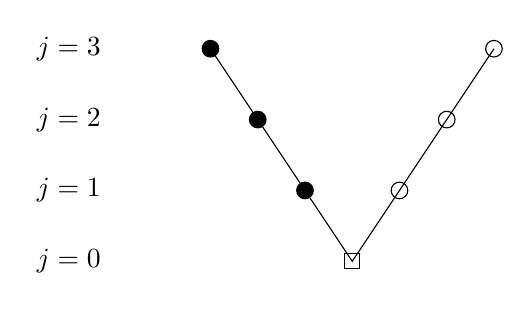
\begin{tikzpicture}[scale=1.2]
  \pgfmathsetmacro\hstep{0.5}
  \pgfmathsetmacro\vstep{0.75}
  \pgfmathsetmacro\ceps{0.08}   % size of square for coarse grid

% grid labels at left
  \node at (-2,3*\vstep) {$j=3$};
  \node at (-2,2*\vstep) {$j=2$};
  \node at (-2,\vstep) {$j=1$};
  \node at (-2,0.0) {$j=0$};

% V-cycle
  \draw[black,thin] (-\hstep,3*\vstep) -- (0.0,2*\vstep) -- (\hstep,\vstep) --  (2*\hstep,0.0)
                    -- (3*\hstep,\vstep) -- (4*\hstep,2*\vstep) -- (5*\hstep,3*\vstep);
  \filldraw (-\hstep,3*\vstep) circle (2.5pt);
  \filldraw (0.0,2*\vstep) circle (2.5pt);
  \filldraw (\hstep,\vstep) circle (2.5pt);
  \draw     (2*\hstep-\ceps,-\ceps) rectangle (2*\hstep+\ceps,+\ceps);
  \draw     (3*\hstep,\vstep) circle (2.5pt);
  \draw     (4*\hstep,2*\vstep) circle (2.5pt);
  \draw     (5*\hstep,3*\vstep) circle (2.5pt);
\end{tikzpicture}

\caption{A four-level V-cycle with distinguished methods: down-smoother (solid dots), up-smoother (circles), and coarse-level solver (square).}
\label{fig:vcycle}
\end{figure}

To summarize this fundamental algorithm (Figure \ref{fig:vcycle}), after ``down-smoother'' sweeps, here denoted $\text{\textsc{smoother}}^{\text{\texttt{down}}}$, the correction equation \eqref{eq:coarsecorrection} is applied on the next-coarser level with a ``new'' source (linear functional) $\ell^{j-1}$, and a zero initial iterate.  Observe that $\ell^{j-1}$ is the amount by which the finer-level iterate $w^j$ did not already solve the problem; for example, if $w^J=u^h$ then $\ell^{J-1}=0$.  After the correction additional ``up-smoother'' sweeps are done to remove high-frequency components from the updated iterate.  Note that memory is needed to hold the states $w^0,\dots,w^J$ (i.e.~until after all coarse-level corrections).  It is also common to implement \pr{gmg-vcycle} recursively.

The default settings give a V-cycle, denoted V(1,1).  If \id{up} $=0$ we get a V(1,0) down-slash cycle and \id{down} $=0$ gives a V(0,1) up-slash (Figure \ref{fig:msccycles}).

The algorithm calls a solver subroutine on the coarsest $j=0$ level.  This may be a direct solver for a linear problem, but they are not available for our nonlinear glacier problems.  For simplicity and generalizability we suppose \pr{gmg-coarsesolve} is also implemented as a fixed number of in-place smoother sweeps:
\begin{pseudo*} \label{ps:gmg-coarsesolve}
\pr{gmg-coarsesolve}(w,F,\id{coarse}=1)\text{:} \\+
    $\text{\pr{smoother}}^{\text{\id{coarse}}}(0,w,F)$ \\
\end{pseudo*}
If the coarsest mesh has a single node ($m_0=1$) then, for a linear problem, a single sweep exactly solves the $j=0$ problem.  In general, an accurate solution is fast if $m_0$ is small, but the choice of a coarse-level mesh and solver is nontrivial for realistic problems (sections \ref{sec:sia} and \ref{sec:stokes}).

Before proceeding, the reader might ask what makes the above V-cycles ``geometric''?  Though the label is partly historical, note that our restriction and prolongation operators arise from the dimensions of the FE mesh via coefficients which use the hat functions ($c_{pq} = \psi_p^{j-1}(x_q^j)$).  Also, we \emph{rediscretize} on coarser levels, that is, we use the original bilinear form $a(\cdot,\cdot)$ on all levels.  An alternative to rediscretization is the \emph{Galerkin} approach which forms coarser-level matrices recursively by $A^{j-1} = R A^j P$, starting from $A^J$ which is the fine-level system matrix; see \cite[Chapter V]{Braess2007} and \cite[Chapter 6]{Bueler2021}.  Going further away from our approach, in a \emph{algebraic multigrid} (AMG) method \cite[Appendix A]{Trottenbergetal2001} the prolongation $P$ is constructed using operations on the entries of $A^J$, and such algorithms invariably define $R=P^\top$.  On linear elliptic problems the geometric and algebraic approaches are closely-related, in part because AMG has been ``tuned'' to generate prolongations $P$ with similar coefficients, but for our upcoming nonlinear and inequality-constrained problems the geometric approach generalizes directly.  By contrast, AMG can only solve the linear steps in a separately-constructed iteration, e.g.~by requiring an outer Newton iteration.  GMG and AMG approaches are natural competitors for the highest-performance solutions, but we will persevere here with the geometric approach.

\subsection*{On transfer operators}  The operators $R$ and $P$ make no choices, which is the meaning of ``canonical''.  However, their application requires computation because of how we represent functions and functionals on each level.  In fact, full-weighting formulae \eqref{eq:canonicalrestrictionaction} and \eqref{eq:canonicalprolongationaction}, which generalize verbatim to unstructured 2D and 3D meshes when the indices $p,q$ denote the nodes of the mesh \cite[Chapter V]{Braess2007}, arise from the simple fact \eqref{eq:hatcombination}, that each coarse-level hat function is a linear combination of fine-level hats.

As linear operators, $R$ and $P$ may be represented as sparse, rectangular matrices, and they are transposes ($P=R^\top$), but using memory to store them this way is unnecessary.  They are applied in $O(m_j)$ operations via \eqref{eq:canonicalrestrictionaction} and \eqref{eq:canonicalprolongationaction}.

Note the two operators differ in their invertibility.  The one-to-one map $P$ has a left inverse.  Said differently, function $y$ in $\mathcal{V}^{j-1}$ can be exactly recovered from $Py$ because they are the same piecewise-linear function, and indeed we will only explicitly write $P$ when indicating a change in vector representation.  By contrast, $\ell$ in $(\mathcal{V}^j)'$ is not recoverable from $R\ell$ because the values $\ell[\psi_q^j]$, i.e.~the action of $\ell$ on the finer level hats, are averaged onto the coarse level and lost.

It turns out that four such mesh-level \emph{transfer} operators are used in this paper (Table \ref{tab:transfers}), but the other two are only introduced in the next section.

\newcommand{\iP}{P^{\hookrightarrow}}
\begin{table}
\begin{tabular}{l|ccccc}
\emph{operator}              & \emph{equation}  & \emph{domain}          & \emph{range}
                  & \emph{one-to-one} & \emph{linear} \\ \hline
canonical prolongation $P$   & \eqref{eq:canonicalprolongationaction} & $\mathcal{V}^{j-1}$    & $\mathcal{V}^j$
                  & \checkmark & \checkmark \\
solution prolongation $\hat P$   & \eqref{eq:solutionprolongation} & $\mathcal{V}^{j-1}$    & $\mathcal{V}^j$
                  &            &  \\
canonical restriction $R$    & \eqref{eq:canonicalrestrictionaction} & $(\mathcal{V}^j)'$     & $(\mathcal{V}^{j-1})'$
                  &            & \checkmark \\
monotone restriction $\mR$   & \eqref{eq:monotonerestriction} & $\mathcal{V}^j$        & $\mathcal{V}^{j-1}$
                  &            &            \\
\end{tabular}

\medskip
\caption{We use four transfer operators in this paper.  The nonlinear $\mR$ and $\hat P$ operators are defined in section \ref{sec:obstacle}.}
\label{tab:transfers}
\end{table}

We have now presented a basic GMG algorithm for linear PDEs via a particular FE viewpoint, namely the MSC approach pioneered by Xu \cite{Xu1992} and others.  The MSC viewpoint is foundational for multilevel, domain-decomposition, and other advanced algorithms \cite[for example]{Farrelletal2019}.  Our next step might be to show computational results demonstrating the efficiency of a GMG algorithm, giving evidence of optimal $O(m_J)$ time to solve the problem, and indeed such results appear in all of our multigrid references \cite{Braess2007,Briggsetal2000,Bueler2021,Elmanetal2014,Trottenbergetal2001}.  However, we first introduce a less-standard ``obstacle'' problem because it shows the essential free-boundary character of the glacier geometry problem.  Computational results appear in each of the next three sections.


\section{Constraint decomposition for the obstacle problem} \label{sec:obstacle}

\subsection*{An ice-like model problem}  We now have a clear view of the GMG method, for a linear equation and from the MSC point of view.  However, as addressed in section \ref{sec:intro}, the main problem of how glacier geometry and ice velocity co-evolve in response to climatic inputs requires an inequality constraint for well-posedness.  The fact that the ice surface elevation is above the bed generates the land-terminating mass-conservation boundary condition.  This constraint, by itself, makes the problem nonlinear and reduces solution regularity, making it challenging to numerical methods.

To address such constraints in a multilevel framework, and before actually modeling glaciers in section \ref{sec:sia}, we introduce the \emph{classical obstacle problem}.  It simply adds an inequality constraint to linear Poisson equation \eqref{eq:poisson}.  After stating the weak form, which is now solved over a convex \emph{subset} of the function space, we will modify the MSC approach into the \emph{multilevel constraint decomposition} (MCD) method.  Each mesh level will host an inequality-constrained problem, and together all the levels will capture the constraint subset.  The nonlinear SIA model (section \ref{sec:sia}) and the Stokes model (section \ref{sec:stokes}) will use a nonlinear extension of the MCD method.

Consider the same 1D domain and solution space $\mathcal{H}=H_0^1[0,1]$ as before.  Let $\varphi(x)$ be a fixed function, the obstacle, from $\mathcal{H}$.  The strong form of the classical obstacle problem is the following \emph{complementarity problem} (CP) \cite{Bueler2021,KinderlehrerStampacchia1980} which says that the solution $u(x)$ is above $\varphi(x)$ \emph{and} that a differential equation applies whereever $u$ is strictly above $\varphi$:
\begin{align}
  u - \varphi &\ge 0 \label{eq:obstaclecp} \\
  -(\alpha u')'-f &\ge 0 \notag \\
  (u-\varphi)(-(\alpha u')'-f) &= 0 \notag
\end{align}
The third condition, \emph{complementarity} itself, implies that for each $x$ in $[0,1]$ the solution either coincides with the obstacle ($u(x)=\varphi(x)$) or PDE \eqref{eq:poisson} holds.  (Both facts can hold at $x$, but in the generic \emph{nondegenerate} \cite{KinderlehrerStampacchia1980} case the obstacle does not itself solve the PDE.)

In the $u=\varphi$ region the constraint is said to be \emph{active}, while \eqref{eq:poisson} holds in the \emph{inactive} portion where $u>\varphi$.  One refers to PDE \eqref{eq:poisson} as the \emph{interior condition} of the CP \cite{KinderlehrerStampacchia1980}.  Note that in the active region the source term is bounded above, $u=\varphi \implies f \le -(\alpha\varphi')'$, but the corresponding statement does \emph{not} hold for the glacier problems in sections \ref{sec:sia} and \ref{sec:stokes}.

Simply by choosing a source term $f(x)$ which is positive in the middle of the domain and negative near the boundaries, we create an ``ice-like'' solution to \eqref{eq:obstaclecp}.  For example, Figure \ref{fig:icelike} (top) shows the exact, piecewise-quadratic solution $u(x)$ for the following data:
\begin{equation}
\varphi(x) = x(1-x), \quad \alpha(x)=1, \quad f(x) = \begin{cases} 8, & 0.2 < x < 0.8, \\
                                                                 -16, & x<0.2 \text{ or } x>0.8. \end{cases}  \label{eq:icelikedetails}
\end{equation}
(Note that $f$ is in $L^2[0,1]$ and is defined almost everywhere.)  Finding the exact formula for $u(x)$, which smoothly-connects five quadratic pieces, is an exercise for the reader.\footnote{Solution in\, \href{https://github.com/bueler/mg-glaciers/blob/master/py/obstacle.py}{\texttt{github.com/bueler/mg-glaciers/blob/master/py/obstacle.py}}.}  The bottom Figure shows a more typical solution for illustrating obstacle problems \cite[for example]{Bueler2021,Tai2003}.

% regenerate:
%   $ cd py/1D/
%   $ ./obstacle.py -plain -jfine 7 -o icelike.pdf
%   $ ./obstacle.py -plain -jfine 7 -o parabola.pdf -problem parabola
%   $ pdfcrop icelike.pdf icelike.pdf
%   $ pdfcrop parabola.pdf parabola.pdf
\begin{figure}
\,\,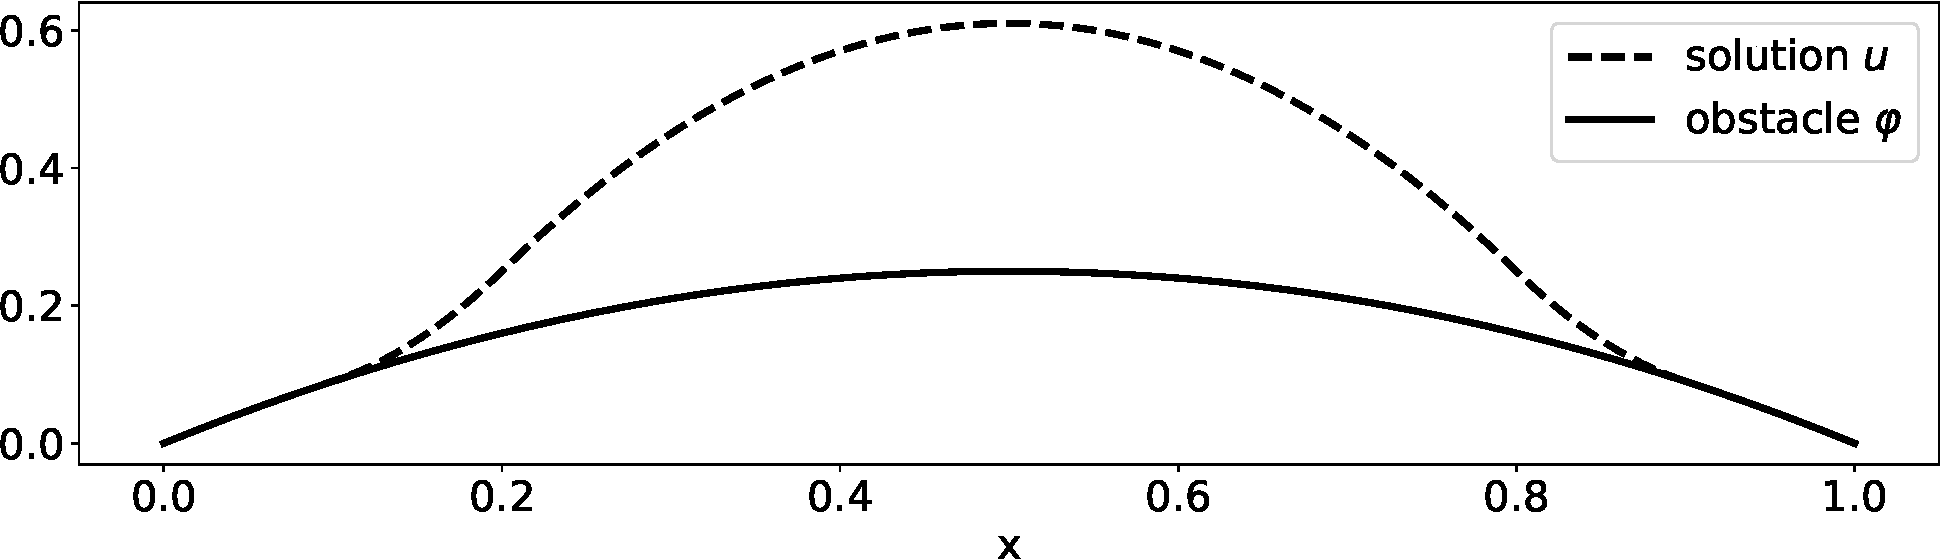
\includegraphics[width=0.8\textwidth]{fixfigs/icelike.pdf}

\bigskip\medskip
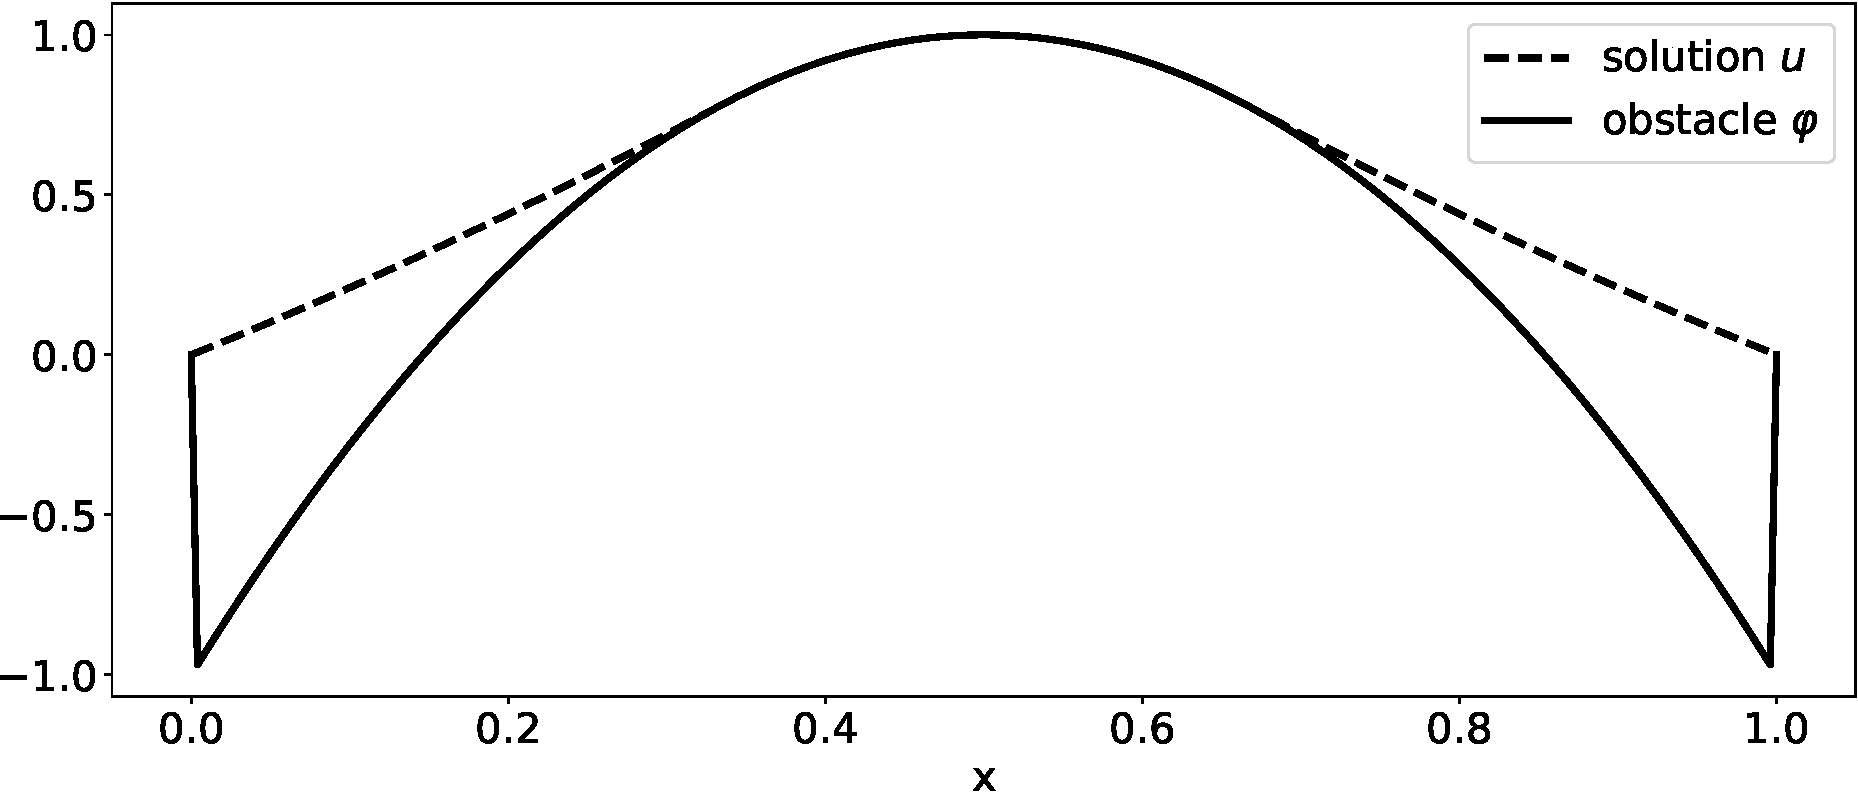
\includegraphics[width=0.82\textwidth]{fixfigs/parabola.pdf}

\medskip
\caption{\emph{Top:} An ice-like configuration of the classical obstacle problem, with $f$ of both signs. \emph{Bottom:} A traditional configuration with $f=0$.}
\label{fig:icelike}
\end{figure}

Unlike problem \eqref{eq:poisson}, the solution to \eqref{eq:obstaclecp} does \emph{not} depend linearly on the source function $f$.  For example, if $f \le 0$ and the obstacle is concave-down ($\varphi'' \le 0$) then the solution is $u=\varphi$.  (By the maximum principle \cite{Evans2010} there are no inactive points in this case.)  In such a case, if $\tilde u$ solves the problem for $\tilde f$ then $2\tilde u$ does not solve the problem for source term $2\tilde f$.  In this sense the classical obstacle problem is nonlinear even though its interior condition PDE is linear.

The glacier problem also has a CP formulation (section \ref{sec:sia}; see also \cite{Calvoetal2002}) in which the obstacle is the bed elevation, the solution is the glacier surface elevation, and the source term is the surface mass balance.  In the inactive region, i.e.~on the glacier, the mass conservation equation applies, and the surface mass balance must be negative in the active region off the glacier.

\subsection*{Weak formulation with constraints}  We now define a closed subset which incorporates the constraint:
\begin{equation}
\mathcal{K} = \left\{v \ge \varphi\right\} \subseteq \mathcal{H}.  \label{eq:Kdefine}
\end{equation}
If $v$ is in $\mathcal{K}$ then we say $v$ is \emph{admissible}.  Note $\mathcal{K}$ is not a vector space, but it is \emph{convex}, that is, if $v,w$ are in $\mathcal{K}$ then any point on the line segment connecting them, $\theta v + (1-\theta) w$ for $0 \le \theta \le 1$, is also in $\mathcal{K}$.  One should also observe that $\mathcal{K}$ is a \emph{cone} with vertex at $\varphi$.  That is, if $v$ is in $\mathcal{K}$ then $\lambda(v-\varphi) + \varphi$ is also in $\mathcal{K}$ for any $\lambda \ge 0$; the ray from $\varphi$ through $v$ is in $\mathcal{K}$.

Derivation of the weak form involves multiplying the strong form \eqref{eq:obstaclecp} by a test function and integrating by parts.  The inequalities enter into the derivation; see \cite[Chapter 12]{Bueler2021}, \cite{JouvetBueler2012}, or \cite{KinderlehrerStampacchia1980} for details.  The result is a single \emph{variational inequality} (VI),
\begin{equation}
  a(u,v-u) \ge \ip{f}{v-u} \quad \text{ for all } v \text{ in } \mathcal{K}, \label{eq:obstaclevi}
\end{equation}
using the same bilinear form $a$ defined in \eqref{eq:weakpoissonearly}.  Recalling \eqref{eq:residual}, the VI can be restated using the residual functional:
\begin{equation}
  F(u)[v-u] \ge 0 \quad \text{ for all } v \text{ in } \mathcal{K}. \label{eq:obstacleviresidual}
\end{equation}

Formulations \eqref{eq:obstaclecp} and \eqref{eq:obstacleviresidual} are equivalent up to the same regularity concerns which relate the strong and weak forms of a PDE.  (See reference \cite{Evans2010} regarding the solution regularity of PDEs, and \cite{KinderlehrerStampacchia1980} for the corresponding VI theory.)  However, some intuition for VIs is needed for understanding the current paper, and so, in an attempt to help, we provide a second weak form.

Inequality \eqref{eq:obstacleviresidual} is equivalent to \emph{constrained minimization} of an \emph{objective} functional $I$:
\newcommand{\argmin}{\mathop{\mathrm{arg\text{-}min}}}
\begin{equation}
  u = \argmin_{w \text{ in } \mathcal{K}} I(w) \quad \text{where} \quad I(w) = \frac{1}{2} a(w,w) - \ip{f}{w}. \label{eq:obstaclemin}
\end{equation}
That is, $u$ is the minimizer, over the constraint set $\mathcal{K}$, of the scalar, quadratic, and \emph{coercive} functional $I$.  (Coercive means that $I(w) \to +\infty$ as $\|w\|_{\mathcal{H}} \to \infty$ \cite{Evans2010}.)  Note that the unconstrained minimum of $I(w)$ over $\mathcal{H}$ may lie outside $\mathcal{K}$.  See Figure \ref{fig:cartoonplane}.

\begin{figure}
\includegraphics[width=0.6\textwidth]{genfigs/cartoonplane.pdf}
\caption{Variational inequality \eqref{eq:obstacleviresidual}, equivalently \eqref{eq:obstaclevigradient}, characterizes the minimum $u$ of $I(w)$ over the shaded convex cone $\mathcal{K}=\{v\ge \varphi\} \subset \mathcal{H}$.  Any vector $v-u$, for $v$ in $\mathcal{K}$, is within $90^\circ$ of $F(u) = \grad I(u)$.}
\label{fig:cartoonplane}
\end{figure}

The (Gateaux) derivative of $I$ is a linear functional in $\mathcal{H}'$:
\begin{equation}
  \grad I(w)[v] = \lim_{\eps\to 0} \frac{I(w+\eps v) - I(w)}{\eps} = a(u,v) - \ip{f}{v}.  \label{eq:gradobjective}
\end{equation}
In fact $\nabla I = F$, the residual, so the VI \eqref{eq:obstacleviresidual} can re-stated yet again:
\begin{equation}
  \nabla I(u)[v-u] \ge 0 \quad \text{ for all } v \text{ in } \mathcal{K}. \label{eq:obstaclevigradient}
\end{equation}

Formulation \eqref{eq:obstaclevigradient} permits a clear, geometrical meaning to the VI, as in the Figure.  The solution $u$ sits at a location in $\mathcal{K}$, often on the boundary, where any vector pointing into the admissible set, namely $v-u$ for $v$ in $\mathcal{K}$, points ``uphill'' on the graph of $I$.  That is, one cannot make minimization progress by moving $u$ to a distinct point $v$ in $\mathcal{K}$.  Identifying $\mathcal{H}$ and its dual space $\mathcal{H}'$, one might write \eqref{eq:obstaclevigradient} as ``$\ip{\nabla I(u)}{v-u} \ge 0$'': the angle between $\nabla I(u)$ and $v-u$ is at most 90 degrees.

The solutions shown in the earlier Figure \ref{fig:icelike} recall what points in $\mathcal{K}$ actually are, namely functions on $[0,1]$.  When a solution $u$ coincides with the obstacle $\varphi$ on a part of the domain then $u$ is on the boundary of $\mathcal{K}$.  In that case arbitrarily-small perturbations $\delta u$, from $\mathcal{H}$, will put $u+\delta u$ outside of $\mathcal{K}$.

The glacier problems in sections \ref{sec:sia} and \ref{sec:stokes} will be formulated both as CPs like \eqref{eq:obstaclecp} and VIs like \eqref{eq:obstacleviresidual}.  However, for general bed elevation functions (obstacles) the glacier problem has no constrained minimization formulation like \eqref{eq:obstaclemin}, so the VI formulations have no interpretation like \eqref{eq:obstaclevigradient}.  The essential reason is the lack of a symmetry of the weak form; see \cite{JouvetBueler2012} for the argument in the SIA case.  However, for glacier problems we at least possess a map $F$, from $\mathcal{K}$ to $\mathcal{H}'$, and if $u$ solves the VI then, heuristically, $F(u)$ points perpendicularly into $\mathcal{K}$.  We may visualize the general VI form \eqref{eq:obstacleviresidual} essentially as in Figure \ref{fig:cartoonplane}, but without the contours of $I$ or the identification of $F$ as a gradient.

Regardless of how the classical obstacle problem is formulated, a \emph{free boundary} generally arises in the interior of the domain.  For example, on either side of the midpoint in Figure \ref{fig:icelike} there are locations where the solution first comes fully in contact with the obstacle.  At these locations both $u=\varphi$ and $u'=\varphi'$ hold, that is, the solution is tangent to the obstacle at the free boundary.  These simultaneous Dirichlet and Neumann conditions occur at a location which must be found as part of the solution; they characterize the free boundary \cite[Chapter V]{KinderlehrerStampacchia1980}.  The analogous conditions in the glacier problem are that both the ice thickness and the horizontal ice flux go to zero at a grounded glacier margin \cite{Bueler2016,JouvetBueler2012}.

The solution of the classical obstacle problem will generally be non-smooth at a free boundary even when the data are arbitrarily smooth.  For example, smoothing the source term $f$ in \eqref{eq:icelikedetails} by ``mollification'' \cite{Evans2010}, so that the transition between positive and negative values would be $C^\infty$, would give a solution nearly the same as shown in Figure \ref{fig:icelike} (top).  However, the free boundary would remain, and at that free boundary the second derivative $u''$ would jump discontinuously from value $+16=-f$ to value $-2=\varphi''$.  A similar jump in $u''$ applies at the free boundary in Figure \ref{fig:icelike} (bottom), from $0=f$ to $-16=\varphi''$.  In general it is known that for smooth $C^\infty$ data ($f,\varphi$) the obstacle problem solution $u$ is in the Sobolev space $W^{2,\infty}$, but it is not in $C^2$ \cite[section IV.6]{KinderlehrerStampacchia1980}.

\subsection*{Smoothers: projected Gauss-Seidel and Jacobi}  Now consider the FE method for a VI.  On each mesh level we will define an obstacle $\phi^j$ in $\mathcal{V}^j$, an admissible set $\mathcal{K}^j = \{v \ge \phi^j\} \subset \mathcal{V}^j$, and a residual function $F^j$.  (Recall $\mathcal{V}^j$ is the vector space spanned by the $j$th-level hats $\psi_p^j$; see section \ref{sec:subspace}.)  The FE method seeks $y^j$ in $\mathcal{K}^j$ so that a finite-dimensional VI holds:
\begin{equation}
  F^j(y^j)[v-y^j] \ge 0 \quad \text{ for all } v \text{ in } \mathcal{K}^j. \label{eq:feobstacleviresidual}
\end{equation}

If we were to solve on the fine-level only, i.e.~in a single-level method, then we would choose the obstacle $\phi^J$ to be the piecewise-linear interpolant of the continuum obstacle $\varphi$, i.e.~$\phi^J=\varphi^J$, and $F^J$ as the original residual $F(w)[\cdot] = a(w,\cdot) - \ip{f}{\cdot}$.  However, in our multilevel method the constructions of $\phi^j$ and $F^j$ will be nontrivial, including on the finest level.  We will have much more to say regarding the obstacles $\phi^j$, but we will write the residual in the form $F^j(w)[\cdot] = a(w,\cdot) - \ell^j[\cdot]$ for some $\ell^j$ in $(\mathcal{V}^j)'$.

Before addressing the multilevel method we propose an iterative method for solving \eqref{eq:feobstacleviresidual}, namely \emph{projected Gauss-Seidel} (PGS) as a smoother.  Supposing $w$ in $\mathcal{K}^j$ is any iterate, the smoother modifies $w$ at the $p$th node so that \eqref{eq:feobstacleviresidual} holds ``at'' that node, but note that if $w$ is admissible then $w+c\psi_p^j$ is admissible if and only if $w_p + c \ge \phi_p$ where $\phi_p = \phi^j(x_p^j)$.  (\emph{Warning.}  This equivalence holds for piecewise-linear elements, but not generally for higher-order polynomial elements.)  For clarity we describe PGS using the constrained minimization form \eqref{eq:obstaclemin}, using a convex scalar function based on the objective functional.  Let
\begin{equation}
i(b) = I^j(w+b\psi_p^j),
\end{equation}
where $I^j(w) = \frac{1}{2} a(w,w) - \ell^j[w]$ and $b$ is a real number.  At each point $p$ we seek the minimizer over admissible perturbations,
\begin{equation}
  c = \argmin_{b \ge \phi_p - w_p} \, i(b).  \label{eq:pgsminimization}
\end{equation}
The minimum of $i(b)$ on the admissible interval $\phi_p - w_p \le b < \infty$ occurs either at the critical point $i'(b)=0$ or at the left end of the interval.  Since $i'(b) = F^j(w)[\psi_p^j] + b a(\psi_p^j,\psi_p^j)$,
\begin{equation}
  c = \max\left\{-\frac{F^j(w)[\psi_p^j]}{a(\psi_p^j,\psi_p^j)}, \, \phi_p - w_p\right\}  \label{eq:pgsformula}
\end{equation}
solves \eqref{eq:pgsminimization}.  In other words, we compute the critical point and project it into the admissible interval.  Then we update $w \gets w + c\psi_p^j$ and proceed to the next point.

This minimization view of PGS is not essential, however.  We can derive formula \eqref{eq:pgsformula} using only VI \eqref{eq:feobstacleviresidual} as follows.  We seek $c$ such that $w+c\psi_p^j$ is admissible and so that \eqref{eq:feobstacleviresidual} holds for all admissible $v=w+\tilde c\psi_p^j$.  That is, we find $c\ge \phi_p-w_p$ so that
\begin{equation}
  F^j(w+c\psi_p^j)[(w+\tilde c\psi_p^j) - (w+c\psi_p^j)] = (\tilde c - c) F^j(w+c\psi_p^j)[\psi_p^j] \ge 0,  \label{eq:pgspointwisevi}
\end{equation}
for all $\tilde c\ge \phi_p-w_p$.  Inequality \eqref{eq:pgspointwisevi} is a one-dimensional VI of form $(\tilde c - c)g(c) \ge 0$, on an interval, thus $g(c)=0$ or $c$ is at the end of the interval, and thus \eqref{eq:pgsformula} follows.

The following pseudocode, a small modification of \pr{gs-sweep} on page \pageref{ps:gs-sweep}, implements PGS:
\begin{pseudo*} \label{ps:pgs}
\pr{pgs}(j,w,F,\phi,\id{omega}=1)\text{:} \\+
    \ct{check admissibility: $w\ge \phi$} \\
    for $p=1,\dots,m_j$ \\+
        $c = -F(w)[\psi_p^j] \,\big/\, a(\psi_p^j,\psi_p^j)$ \\
        $w_p \gets \max\{w_p + \id{omega}\,c, \phi_p\}$
\end{pseudo*}

As noted in section \ref{sec:subspace}, GS-type (i.e.~multiplicative) smoothers re-evaluate the residual after each point update.  This is an acceptable $O(1)$ cost when the residual of an iterate at a point $x_p^j$ is computable from a few neighboring values, as applies here and in section \ref{sec:sia}.  However, when the residual is nonlocal, and especially when it is both nonlocal and expensive to evaluate, as for the Stokes-based model in section \ref{sec:stokes}, a GS-type smoother becomes less practical.  An alternative is an additive smoother in which the vector residual is evaluated once at the beginning.  The following modifies \pr{jacobi-sweep} on page \pageref{ps:jacobi-sweep}.
\begin{pseudo*} \label{ps:pjacobi}
\pr{pjacobi}(j,w,F,\phi,\id{omega}=0.67)\text{:} \\+
    \ct{check admissibility: $w\ge \phi$} \\
    $r = F(w)[\cdot]$ \\
    for $p=1,\dots,m_j$ \\+
        $c = -r_p \,\big/\, a(\psi_p^j,\psi_p^j)$ \\
        $w_p \gets \max\{w_p + \id{omega}\,c, \phi_p\}$
\end{pseudo*}
(We could also describe this smoother as a projected forward Euler step (section \ref{sec:subspace}), i.e.~as a step of the common time-evolution method in glacier and ice sheet models \cite[for example]{Winkelmannetal2011}.)  Assuming each pointwise residual $F(w)[\psi_p^j]$ is an $O(1)$ operation in the $j$th-level representation, \pr{pgs} and \pr{pjacobi} are $O(m_j)$ operations.  The latter remains $O(m_j)$ as long as the vector residual and the diagonal entries can be computed in $O(m_j)$ operations given $w$, even if individual pointwise residuals are not $O(1)$.

For appropriate ranges of \id{omega} both algorithms above are known to converge to the solution $y^j$ of VI problem \eqref{eq:feobstacleviresidual} \cite[Proposition 4.5]{GraeserKornhuber2009}, but, of course, slowly on fine meshes.  Regarding the relaxation parameter \id{omega}, recall that the optimal value for the Poisson equation is \id{omega} $=2/3$ \cite{Briggsetal2000}, but finding the most-effective smoother values for obstacle problems is a topic for numerical experimentation.

However, for VI problems the residual norm $\|F(w)\|_2$ does not generally go to zero at the convergence of the iterations.  Recalling the CP formulation \eqref{eq:obstaclecp}, at convergence we have $F(w)[\psi_p^j] = 0$ where $w(x_p^j) > \phi(x_p^j)$ (inactive points), but if $w(x_p^j) = \phi(x_p^j)$ (active points) then $F(w)[\psi_p^j]$ is only required to be nonnegative.  Thus the convergence criterion for iterated PGS sweeps is that the norm of the \emph{CP residual}, the vector
\begin{equation}
  (\hat \bF(w))_p = \begin{cases} F(w)[\psi_p^j], & w_p > \phi_p, \\
                                  \min\{F(w)[\psi_p^j],0\}, & \text{otherwise}, \end{cases} \label{eq:cpresidual}
\end{equation}
in $\RR^{m_j}$, should be small.  Then our relative-norm convergence criterion will be
\begin{equation}
\|\hat\bF(w)\|_2 < \text{\texttt{rtol}}\,\|\hat\bF(w^0)\|_2 \label{eq:cpconvergencecriterion}
\end{equation}
for some tolerance \id{rtol}.

The above projected iterations will serve as our smoothers, applied one or two times on each level, and as the coarse-level solver as well.  However, we are not yet prepared to build a multilevel method for problem \eqref{eq:feobstacleviresidual} because the nontrivial construction of the obstacles $\phi^j$ and residuals $F^j$ remains.  We need to decompose the continuum constraint $\varphi$ across the mesh-level hierarchy, and we need to construct admissible multilevel corrections.

\subsection*{Multilevel constraint decomposition (MCD)}  How do we maintain admissibility throughout a multilevel cycle while not introducing high-frequencies?

Consider the coarse-level correction $e^{j-1}$ in a linear V-cycle (section \ref{sec:subspace}, equation \eqref{eq:coarsecorrection}), which is prolonged onto the $j$th level.  For an obstacle problem the resulting iterate would need to be admissible, i.e.~$w + P e^{j-1}$ would need to be above the obstacle, say $\varphi^j$.  However, as illustrated in Figure \ref{fig:prolongobstacle}, if the obstacles are interpolants of a (common) continuum obstacle $\varphi$ then an iterate which is admissible on the $j-1$ level is \emph{not} necessarily admissible on the $j$ level.  (In the glacier context, a coarse-mesh ice surface may be breached by the fine-mesh bed topography.)  We might try enforcing admissibility by \emph{truncation}, namely overwriting $\tilde w = w + Pe^{j-1}$ with $\max\{\tilde w, \varphi^j\}$.  However, this reintroduces high frequencies, requiring additional smoother effort to remove, and generally damaging multigrid convergence rates.

\begin{figure}
\qquad \includegraphics[width=0.75\textwidth]{genfigs/prolongobstacle.pdf}
\caption{If the obstacles interpolate a common continuum obstacle then an admissible iterate on a coarse level, when prolonged, may not be admissible on a finer level.}
\label{fig:prolongobstacle}
\end{figure}

One way forward is the \emph{multilevel constraint decomposition} (MCD) method of Tai \cite{Tai2003}, described here using the specific decomposition proposed in \cite{GraeserKornhuber2009}.  Suppose $w^J$ in $\mathcal{V}^J$, on the finest level, is admissible in the original sense that
\begin{equation}
  w^J \ge \varphi^J, \label{eq:fineadmissibleiterate}
\end{equation}
where $\varphi^J$ interpolates the continuum obstacle.  Define the \emph{defect constraint} \cite{GraeserKornhuber2009} of $w^J$ as
\begin{equation}
  \chi^J = \varphi^J - w^J.  \label{eq:defectconstraint}
\end{equation}
Note $\chi^J \le 0$.  The meaning of $\chi^J$ is that if we modify $w^J$ by adding $y$ then the result is admissible if and only if $y$ is above $\chi^J$:
\begin{equation}
  w^J + y \ge \varphi^J  \qquad \iff \qquad y \ge \chi^J.  \label{eq:defectmeaning}
\end{equation}

Our MCD method will \emph{put as much of $\chi^J$ into the coarsest levels as possible}.  That is, our decomposition of $\chi^J$ determines how constrained the coarse-level corrections are, and we want to allow the largest corrections on the inexpensive coarse levels.  For this purpose, following \cite[equation (4.22)]{GraeserKornhuber2009}, we define a nonlinear \emph{monotone restriction} operator $\mR$ from $\mathcal{V}^j$ to $\mathcal{V}^{j-1}$.  For $z$ in $\mathcal{V}^j$, $\mR z$ is computed by maximizing nodal values of $z$ over the interior of the support of coarser-level hat functions.  That is, if $z = \sum_q z_q \psi_q^j$ on the fine level then
\begin{equation}
  \mR z = \sum_{p=1}^{m_{j-1}} \zeta_p \psi_p^{j-1} \qquad \text{where} \qquad \zeta_p = \max \{z_q \,:\, \psi_p^{j-1}(x_q^j) > 0\}.  \label{eq:monotonerestriction}
\end{equation}
Observe that $\mR z \ge z$.  Also note that $\mR$ acts on functions $\mathcal{V}^j$ while canonical restriction $R$ acts on linear functionals $(\mathcal{V}^j)'$; see Table \ref{tab:transfers}.

We then define the \emph{$j$th-level defect constraint} inductively by
\begin{equation}
  \chi^j = \mR \chi^{j+1}  \label{eq:chik}
\end{equation}
for $j=J-1$ down to $j=0$.  These defect constraints have two key properties: $\chi^j$ is in $\mathcal{V}^j$ and $\chi^j \ge \chi^{j+1}$.  (One may also write $P \chi^j \ge \chi^{j+1}$.)

The \emph{$j$th-level obstacle} is the difference of defect constraints:
\begin{equation}
  \phi^j = \chi^j - \chi^{j-1} \quad \text{ for } j=0,1,\dots,J,  \label{eq:levelobstacle}
\end{equation}
where we also define $\chi^{-1}=0$ so that $\phi^0 = \chi^0$.  Note $\phi^j$ is in $\mathcal{V}^j$ and $\phi^j\le 0$.

%REGENERATE Figures \ref{fig:gooddecomposition} and \ref{fig:icelikedecomposition}:
%$ ./obstacle.py -jfine 5 -jcoarse 1 -random -randommodes 8 -diagnostics -o defect.pdf
%fine level 5 (m=63): using 20 V(1,0) cycles -> 38.750 WU
\begin{figure}
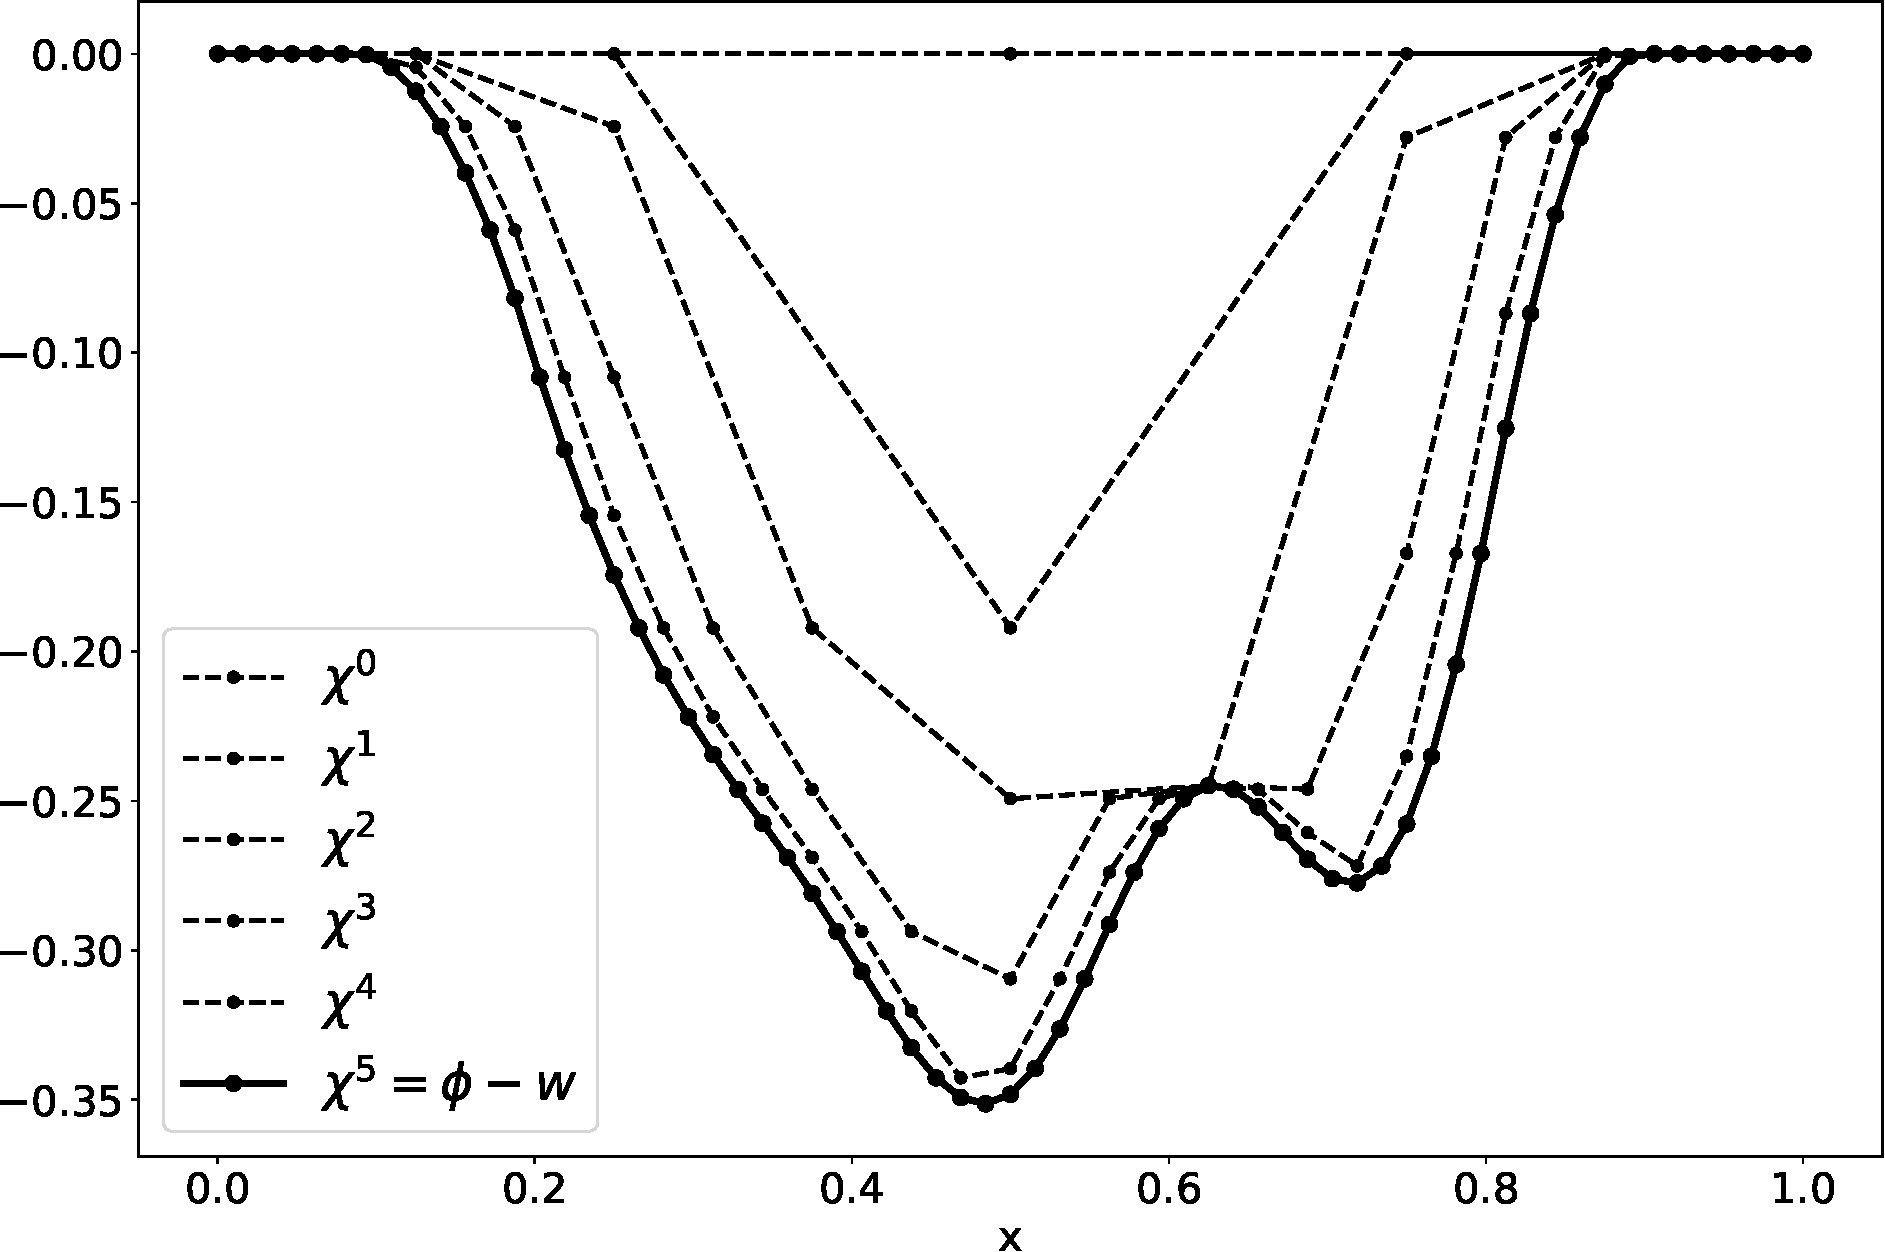
\includegraphics[width=0.75\textwidth]{fixfigs/decomp_defect.pdf}
\caption{Our MCD method writes a fine-level defect constraint $\chi^J = \varphi^J - w^J$ as a sum of obstacles $\phi^j = \chi^j - \chi^{j-1}$ on each level.}
\label{fig:gooddecomposition}
\end{figure}

We have now decomposed the fine-level defect constraint $\chi^J$ via a telescoping sum:
\begin{equation}
  \sum_{j=0}^J \phi^j = \chi^0 + (\chi^1 - \chi^0) + (\chi^2 - \chi^1) + \dots + (\chi^J - \chi^{J-1}) = \chi^J.  \label{eq:telescopingdecomposition}
\end{equation}
An example is shown in Figure \ref{fig:gooddecomposition}.  Note that the obstacles $\phi^j$ are the gaps between the plotted defect constraints $\chi^j$.  If the $J$th level is a high-resolution mesh and the defect constraint $\chi^J$ is smooth then $\phi^J\approx 0$ because $\chi^J$ is well-approximated on the $J-1$ level.

From the obstacles $\phi^j$ we define closed, convex \emph{admissible (correction) sets}
\begin{equation}
\mathcal{K}^j = \left\{v \ge \phi^j\right\} \subseteq \mathcal{V}^j \label{eq:defineKj}
\end{equation}
for $j=0,1,\dots,J$.  Because $\phi^j \le 0$, the zero function is admissible on every level.  On the finest level, note that $\phi^J$ is not the same as $\varphi^J$, and so $\mathcal{K}^J$ does not approximate $\mathcal{K}$.

We also define the $j$th-level \emph{defect constraint set}
\begin{equation}
  \mathcal{D}^j = \left\{v \ge \chi^j\right\} \subset \mathcal{V}^j.  \label{eq:constraintset}
\end{equation}
From the telescoping sum \eqref{eq:telescopingdecomposition}, the admissible correction sets $\mathcal{K}^j$ decompose $\mathcal{D}^j$:
\begin{equation}
  \mathcal{D}^j = \mathcal{K}^0 + \mathcal{K}^1 + \dots + \mathcal{K}^j. \label{eq:constraintdecomposition}
\end{equation}
That is, every $y$ in $\mathcal{D}^j$ can be built by choosing a function from each of the sets $\mathcal{K}^0,\dots,\mathcal{K}^j$.  As with \eqref{eq:subspacedecomposition}, this representation is usually not unique.

Subset equation \eqref{eq:constraintdecomposition} is close to the core meaning of the MCD method.  As shown in Figure \ref{fig:innerconeapprox}, this decomposition implies a nesting of cones:
\begin{equation}
  \mathcal{D}^0 \subset \mathcal{D}^1 \subset \dots \subset \mathcal{D}^J.  \label{eq:nestedcones}
\end{equation}
In particular, the fine-level defect constraint set $\mathcal{D}^J = \{v \ge \chi^J\}$ is approximated ``from within'' by coarser-level cones, the partial sums $\mathcal{D}^j = \sum_{k=0}^j \mathcal{K}^k$.  The smaller sets $\mathcal{K}^j$ are also cones, but they are not nested.  However, though $\mathcal{K}^j$ and $\mathcal{D}^j$ are cone relatives to $\phi^j$ and $\chi^j$, respectively, they are not closed under addition, and therefore corrections must be carefully applied, with attention to admissibility of the new iterate \eqref{eq:defectmeaning}, especially in a V-cycle (see below).

\begin{figure}
\includegraphics[width=0.65\textwidth]{genfigs/innerconeapprox.pdf}

\caption{The MCD method approximates the fine-level defect constraint cone $\mathcal{D}^J = \{v\ge \chi^J\}$ from inside by coarse-level cones $\mathcal{D}^j=\mathcal{K}^0+\dots+\mathcal{K}^j$.}
\label{fig:innerconeapprox}
\end{figure}

Looking forward to the glacier problem in section \ref{sec:sia}, the fine-mesh obstacle $\varphi^J$ will be the bed elevation, $w^J$ will be a candidate ice surface elevation on the fine mesh, and $-\chi^J$ will be the corresponding ice thickness.  With this in mind, Figure \ref{fig:icelikedecomposition} illustrates the same constraint decomposition as in Figure \ref{fig:gooddecomposition}, but pictured as a decomposition of the ``ice'' into layers.  (Compared to Figure \ref{fig:icelike} (top), the ``topography'' $\varphi^J$ here is bumpy.)  However, the earlier Figure plots the decomposition in the correct sense, so that the functions $\chi^j$ and $\phi^j$ are piecewise-linear, and so that the zero correction is admissible on every level.

\begin{figure}
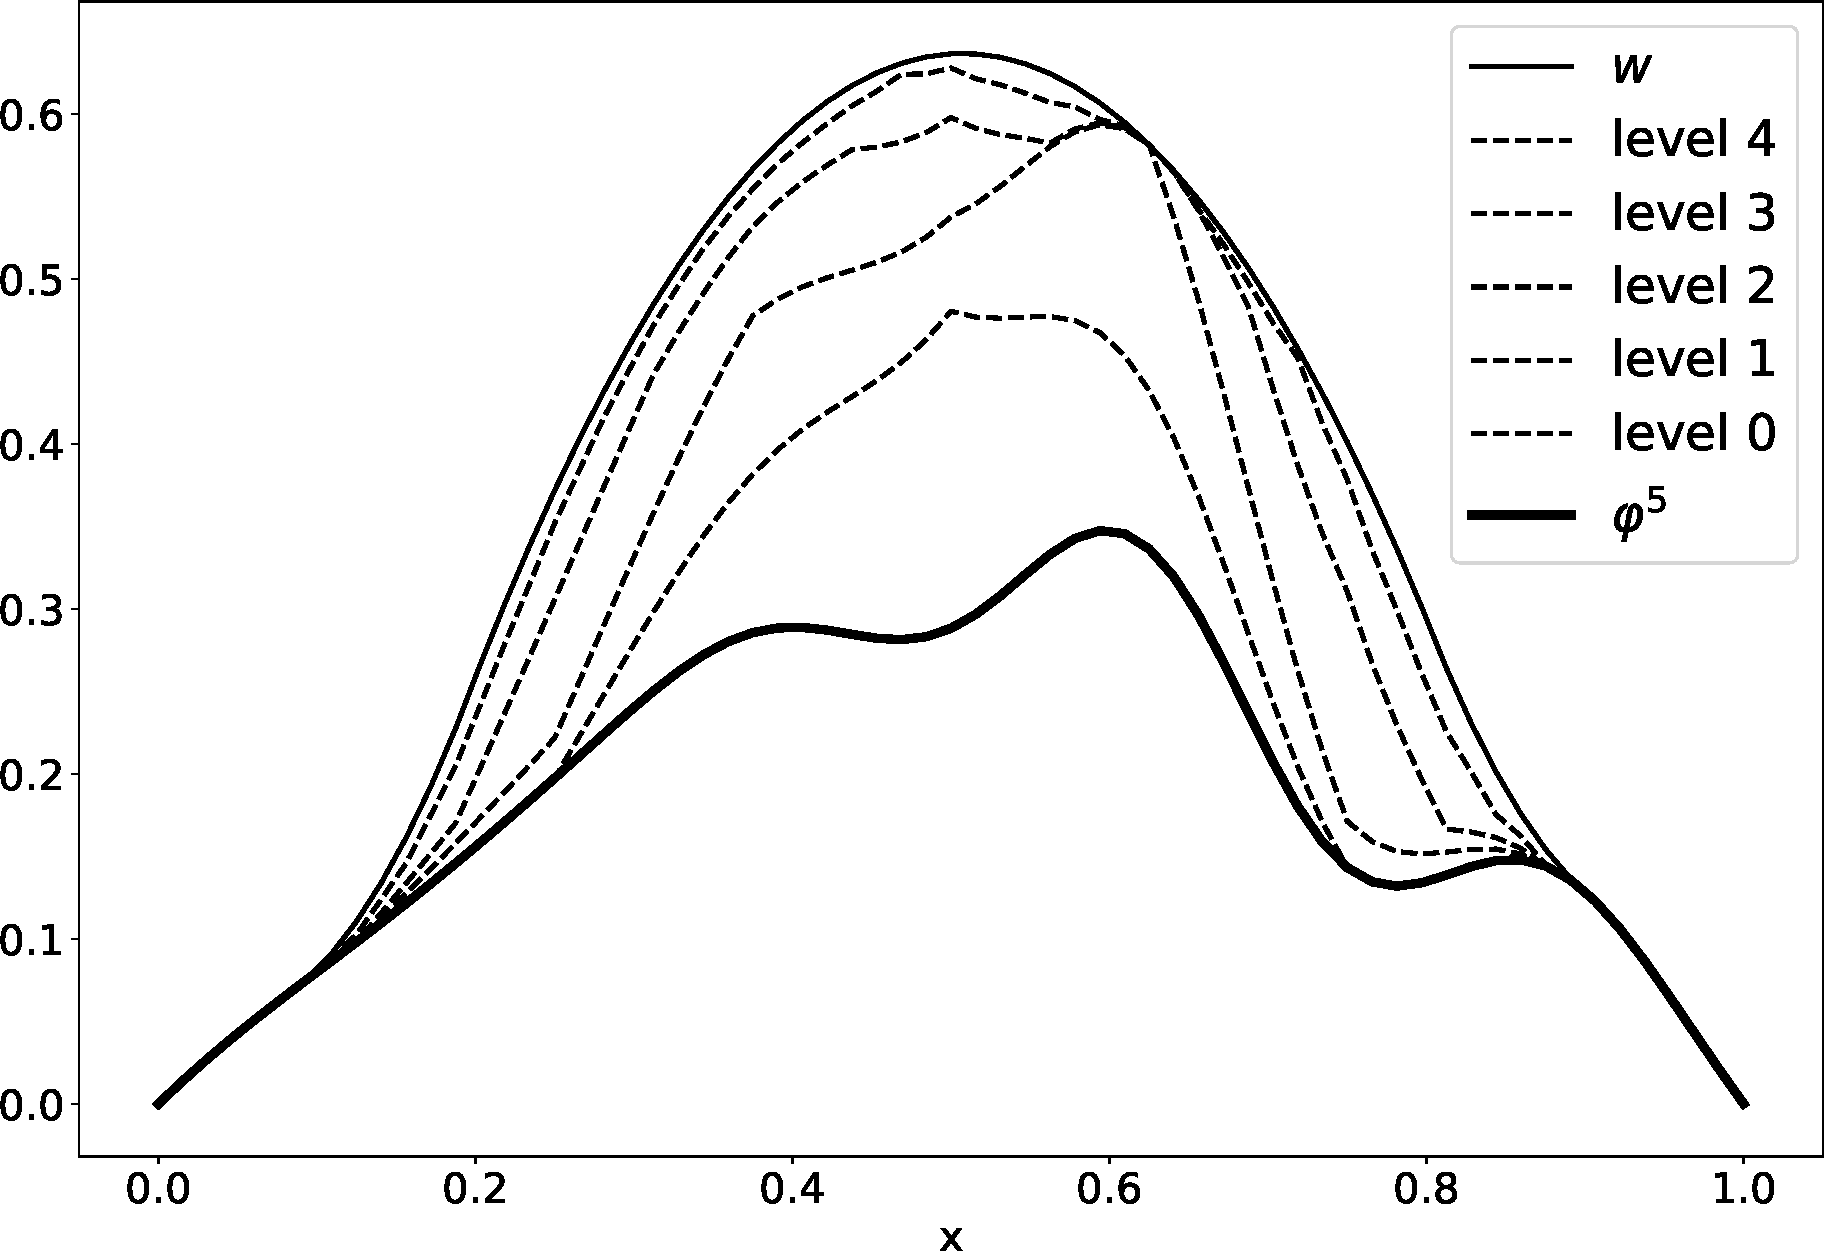
\includegraphics[width=0.7\textwidth]{fixfigs/icedec_defect.pdf}
\caption{A heuristic understanding of Figure \ref{fig:gooddecomposition}: MCD decomposes the ``ice'' between a fine-mesh iterate $w^J$ and the fine-mesh obstacle $\varphi^J$.}
\label{fig:icelikedecomposition}
\end{figure}

\subsection*{MCD coarse-level corrections}  On each mesh level there is now an obstacle problem, and we will write it in three forms.  The forms are equivalent for the classical obstacle problem, but only one will generalize to the glacier problems in sections \ref{sec:sia} and \ref{sec:stokes}.  For now, recall that $F(w)[v] = a(w,v) - \ip{f}{v}$ denotes the continuum residual \eqref{eq:residual}, and then $I(v) = \frac{1}{2} a(v,v) - \ip{f}{v}$ is the corresponding objective function.

Again suppose $w^J$ is an admissible iterate on the fine level: $w^J\ge \varphi^J$.  Assume that we have already descended from the fine level $J$ to some level $j+1$, computing admissible corrections $y^k$ from each set $\mathcal{K}^k=\{v\ge \phi^k\}$, for $k\ge j+1$.  From the definitions of $\chi^J$ and $\mathcal{D}^J$, the function $z = w^J+y^J+\dots+y^{j+1}$ is admissible in the original sense, i.e.~$z\ge \varphi^J$.  The MCD \emph{coarse-level correction} is a function $y$ in $\mathcal{K}^j=\{v\ge \phi^j\}$ such that one of the following holds:
\begin{itemize}
\item general variational inequality \cite{Tai2003}:
\begin{equation}
  F(w^J+y^J+\dots+y^{j+1}+y)[v - y] \ge 0 \qquad \text{for all } v \text{ in } \mathcal{K}^j.  \label{eq:mcdvi}
\end{equation}
\item constrained minimization \cite{Tai2003}:
\begin{equation}
  y = \argmin_{v \text{ in } \mathcal{K}^j} I(w^J+y^J+\dots+y^{j+1}+v).  \label{eq:mcdminimization}
\end{equation}
\item linear variational inequality \cite{GraeserKornhuber2009}:
\begin{equation}
  F^j(y)[v - y] \ge 0 \qquad \text{for all } v \text{ in } \mathcal{K}^j.   \label{eq:mcdvilinear}
\end{equation}
\end{itemize}
In the first form $F$ does not need to be linear, and similarly $I$ in the second form does not need to be quadratic.  Note that this initial description of the problem defines a down-slash cycle (see Figure \ref{fig:msccycles}), but we will show how to generalize to a V-cycle.  In any case a coarse-level correction $y$ in $\mathcal{K}^j$ is defined for every level in the hierarchy, $j=0,\dots,J$.

The third form \eqref{eq:mcdvilinear} exploits linearity of $F$ to inductively define residual functionals which do not directly refer to the fine-level admissible states $z^j = w^J+y^J+\dots+y^{j+1}+y$:
\begin{align}
  F^j(y)[\cdot] &= F(z^j)[\cdot] \label{eq:residuallinearlevelderive} \\
                &= a(w^J+y^J+\dots+y^{j+1}+y,\cdot) - \ip{f}{\cdot} \notag \\
                &= a(y,\cdot) + F^{j+1}(y^{j+1})[\cdot]. \notag
\end{align}
That is, we construct each new source term,
\begin{equation}
  \tilde\ell^j[\cdot] = \begin{cases} - F^{j+1}(y^{j+1})[\cdot], & j < J, \\
                                      - F(w^J)[\cdot],   & j = J, \end{cases} \label{eq:rhslinearlevel}
\end{equation}
thereby define a residual functional on each level,
\begin{equation}
  F^j(y)[\cdot] = a(y,\cdot) - \tilde\ell^j[\cdot].  \label{eq:residuallinearlevel}
\end{equation}
Here $F^j$ is actually defined on $\mathcal{V}^h$, that is, on the whole FE space, and $\tilde\ell^j$ is in $(\mathcal{V}^h)'$.  However, smoothing will occur before each coarse correction, and so we will use the canonical restriction to approximate $\tilde\ell^j$ by a linear functional $\ell^j$ in the coarse-level space $(\mathcal{V}^j)'$; see \eqref{eq:restrictedrhslinearlevel} below.

For the classical obstacle problem, wherein the residual $F(w)[v]$ is built from a symmetric bilinear form $a(w,v)$, the three problems \eqref{eq:mcdvi}--\eqref{eq:mcdvilinear} are equivalent:
   $$\eqref{eq:mcdvilinear} \quad \stackrel{a \text{ bilinear}}{\iff\strut} \quad \eqref{eq:mcdvi} \quad \stackrel{F=\grad I}{\iff\strut} \quad \eqref{eq:mcdminimization}.$$
The left equivalence depends on linearity, and the right on symmetry, but VI form \eqref{eq:mcdvi} in the middle is the most general.  It is the one we will apply for glacier problems.

When $F$ is not the gradient of a coercive objective function, e.g.~as in the SIA and Stokes glacier problems, additional structural properties of $F$ are required for well-posedness (e.g.~monotonicity \cite{Bueler2020,JouvetBueler2012,KinderlehrerStampacchia1980}).  However, we will assume well-posedness and proceed with the numerics.

\subsection*{MCDL cycles}  Now we may implement multilevel cycles for the classical obstacle problem.  Because the interior PDE of this problem is the linear Poisson equation, we solve form \eqref{eq:mcdvilinear} and name the method \pr{MCDL}, with L for ``linear''.  A general nonlinear MCD algorithm is applied to glacier problems in sections \ref{sec:sia} and \ref{sec:stokes}.

We represent functions and linear functionals in the piecewise-linear spaces $\mathcal{V}^j$ and $(\mathcal{V}^j)'$ just as in section \ref{sec:subspace}.  To address how the correction problem is actually moved onto the coarser level, note that equations \eqref{eq:rhslinearlevel} and \eqref{eq:residuallinearlevel} will be applied after smoothing of the previous correction $y^{j+1}$, so we approximate the residual by applying canonical restriction,
\begin{equation}
\ell^j[\cdot] = R \tilde\ell^j[\cdot] = \begin{cases} - R(F^{j+1}(y^{j+1}))[\cdot], & j < J, \\
                                                      - F(w^J)[\cdot],   & j = J, \end{cases} \label{eq:restrictedrhslinearlevel}
\end{equation}
and then we define $F^j(y)[\cdot] = a(y,\cdot) - \ell^j[\cdot]$.  In using $\ell^j$ instead of $\tilde\ell^j$ we lose any high-frequency residual information in $y^{j+1}$ which remains after smoothing.

Implementing formulae \eqref{eq:defectconstraint}, \eqref{eq:chik}, \eqref{eq:levelobstacle}, \eqref{eq:defineKj}, \eqref{eq:mcdvilinear}, and \eqref{eq:restrictedrhslinearlevel} produces a V(1,0) down-slash cycle, namely Algorithm 4.7 in \cite{GraeserKornhuber2009}.

However, once all the corrections $y^j$ are computed on the way down, admissible up-smoothing is more forgiving.  For instance, if we have computed $y^1$ in $\mathcal{K}^1$ and $y^0$ in $\mathcal{K}^0$ then prolongation and accumulation gives $\tilde z = P y^0 + y^1$ in $\mathcal{D}^1 = \mathcal{K}^0 + \mathcal{K}^1$, which we may smooth to $z^1$ in $\mathcal{D}^1$.  In other words, obstacles $\phi^j$ can be regarded as the down-obstacles while the defect constraints $\chi^j$ are the up-obstacles; see Figure \ref{fig:mcdvcycle}.  The observation of this asymmetry permits a better algorithm.  (It also justifies some of the complexity of notation in the previous subsection.)

\begin{figure}
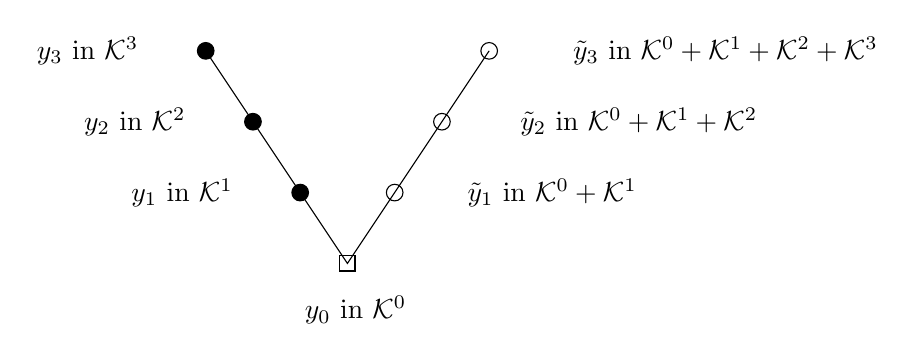
\begin{tikzpicture}[scale=1.2]
  \pgfmathsetmacro\hstep{0.5}
  \pgfmathsetmacro\vstep{0.75}
  \pgfmathsetmacro\ceps{0.08}   % size of square for coarse grid

% V-cycle with MCD down-obstacle and up-obstacle annotations
  \draw[black,thin] (-\hstep,3*\vstep) -- (0.0,2*\vstep) -- (\hstep,\vstep) --  (2*\hstep,0.0)
                    -- (3*\hstep,\vstep) -- (4*\hstep,2*\vstep) -- (5*\hstep,3*\vstep);
  \filldraw (-\hstep,3*\vstep) node[xshift=-15mm] {$y_3$ in $\mathcal{K}^3$} circle (2.5pt);
  \filldraw (0.0,2*\vstep) node[xshift=-15mm] {$y_2$ in $\mathcal{K}^2$} circle (2.5pt);
  \filldraw (\hstep,\vstep) node[xshift=-15mm] {$y_1$ in $\mathcal{K}^1$} circle (2.5pt);
  \draw     (2*\hstep-\ceps,-\ceps) node[xshift=2mm,yshift=-5mm] {$y_0$ in $\mathcal{K}^0$} rectangle (2*\hstep+\ceps,+\ceps);
  \draw     (3*\hstep,\vstep) node[xshift=20mm] {$\tilde y_1$ in $\mathcal{K}^0 + \mathcal{K}^1$} circle (2.5pt);
  \draw     (4*\hstep,2*\vstep) node[xshift=25mm] {$\tilde y_2$ in $\mathcal{K}^0 + \mathcal{K}^1 + \mathcal{K}^2$} circle (2.5pt);
  \draw     (5*\hstep,3*\vstep) node[xshift=30mm] {$\tilde y_3$ in $\mathcal{K}^0 + \mathcal{K}^1 + \mathcal{K}^2 + \mathcal{K}^3$} circle (2.5pt);
\end{tikzpicture}

\caption{Going down, \pr{mcdl-vcycle} computes a correction $y_j$ in $\mathcal{K}^j = \{v\ge \phi_j\}$, but its upward-accumulated correction $z_j$ expands into the larger set $\mathcal{D}^j = \{v \ge \chi_j\}$.}
\label{fig:mcdvcycle}
\end{figure}

The following V-cycle pseudocode uses \pr{pgs} or \pr{pjacobi} as the smoother and coarse-level solver.  It takes $F^J$, defined via \eqref{eq:restrictedrhslinearlevel}, as an argument, and not the original $F$; this V-cycle only knows about the fine-level iterate $w^J$ through $F^J$ and $\chi^J$.  The result is a fine-level correction $z^J$; see \pr{mcdl-solver} next.
\begin{pseudo*} \label{ps:mcdl-vcycle}
\pr{mcdl-vcycle}(J,F^J,\chi^J,\id{down}=1,\id{coarse}=1,\id{up}=0)\text{:} \\+
    for $j=J$ downto $j=1$ \\+
      $\chi^{j-1} = \mR \chi^j$ \qquad\qquad\qquad\qquad \ct{up-obstacle} \\
      $\phi^j = \chi^j - P\chi^{j-1}$ \qquad\qquad\qquad\quad \ct{down-obstacle} \\
      $y^j = 0$ \\
      $\text{\pr{smoother}}^{\text{\id{down}}}(j,y^j,F^j,\phi^j)$ \qquad\quad \ct{in-place down-smoothing in $\mathcal{K}^j$} \\
      $\ell^{j-1}[\cdot] := - R (F^j(y^j))[\cdot]$ \qquad\qquad \ct{update and restrict residual} \\
      $F^{j-1}(y)[\cdot] := a(y,\cdot) - \ell^{j-1}[\cdot]$ \\-
    $y^0 = 0$ \\
    $\text{\pr{smoother}}^{\text{\id{coarse}}}(0,y^0,F^0,\chi^0)$ \qquad\quad \ct{coarsest-level correction} \\
    $z^0 = y^0$ \\
    for $j=1$ to $j=J$ \\+
      $z^j = P z^{j-1} + y^{j}$ \qquad\qquad\qquad \ct{prolong and accumulate corrections} \\
      $\text{\pr{smoother}}^{\text{\id{up}}}(j,z^j,F^j,\chi^j)$ \qquad\quad \ct{in-place up-smoothing in $\mathcal{D}^j$} \\-
    return $z^J$
\end{pseudo*}

In agreement with Algorithm 4.7 in \cite{GraeserKornhuber2009}, the default \id{down} and \id{up} settings give a V(1,0) cycle.  However, any V(\id{down},\id{up}) cycle is allowed, and we will test V(1,0), V(0,1), and V(1,1)\footnote{Reference \cite{GraeserKornhuber2009} describes extending from V(1,0) cycles to V(1,1) cycles by splitting the obstacles $\phi^j$, but it is not clear how this should be implemented.  In any case, our implementation allows larger coarse-level corrections.} cycles below.  Also, in the implementation the functions $F^j(y)[\cdot]$ are not passed as functions in the pro\-gramming-language sense.  Rather, assuming a subroutine which evaluates $a(w,v)$ on each level, the linear functional $\ell^{j-1}$ is passed, from which $F^{j-1}$ is constructed in the smoother.

The following in-place solver adds an outer loop which sets-up the fine-level data $\chi^J$ and $F^J$, calls the V-cycle, and checks for convergence.  Note that one must call this solver with an admissible initial iterate; $w=\varphi^J$ is one possibility.  Compare \pr{msc-solver} in section \ref{sec:subspace}.
\begin{pseudo*} \label{ps:mcdl-solver}
\pr{mcdl-solver}(J,w^J,F,\varphi^J,\id{rtol}=10^{-3},\id{cyclemax}=100)\text{:} \\+
    $r_0=\|\hat\bF(w^J)\|$ \qquad\qquad\qquad\qquad\qquad \ct{initial CP residual norm; see \eqref{eq:cpresidual}} \\
    for $s=1,\dots,\id{cyclemax}$ \\+
        $\chi^J = \varphi^J - w^J$ \qquad\qquad\qquad\qquad\quad \ct{fine-level defect constraint} \\
        $\tilde\ell^J[\cdot] := - F(w^J)[\cdot]$ \qquad\qquad\qquad\quad \ct{see \eqref{eq:restrictedrhslinearlevel}} \\
        $F^J(y)[\cdot] := a(y,\cdot) - \tilde\ell^J[\cdot]$ \\
        $w^J\gets w^J+\pr{mcdl-vcycle}(J,F^J,\chi^J)$ \\
        if $\|\hat\bF(w^J)\| \le \id{rtol} \, r_0$ \\+
            break \\--
\end{pseudo*}

\subsection*{Convergence of the numerical error}  All of the pseudocodes in the current section have been implemented in Python.\footnote{At\, \href{https://github.com/bueler/mg-glaciers/}{\texttt{github.com/bueler/mg-glaciers/}} see the \texttt{py/1D/} directory and its \texttt{README.md}.}  Both to verify these implementations, and to demonstrate the differences in numerical error convergence rates between the obstacle problem and the corresponding unconstrained PDE, we use three exact solutions.  The first two are already shown in Figure \ref{fig:icelike}; note that the ``ice-like'' case has a discontinuous source $f$, while ``traditional'' has $f=0$, but both have smooth, parabolic obstacles.  The third ``unconstrained'' exact solution is for the Poisson equation $-u''=f$.  Specifically, the obstacle is low enough so that the inactive set is $(0,1)$, all smoothing steps avoid projection, and $u(x) = x^2(1-x^2)$, $f(x) = 12 x^2-2$, and $\varphi=-1$.

Figure \ref{fig:convergence} shows the numerical error norm $\|u^h-u\|_2$ as a function of mesh spacing $h$ for runs with \id{rtol} $=10^{-7}$.  The convergence rate for ``traditional'' is the best possible, as $O(h^2)$ error is expected (and observed) for unconstrained problems \cite{Elmanetal2014}.  The ``ice-like'' convergence rate is poor here because of the lower regularity of $f$.  Note that the low regularity of obstacle problem solutions will have a greater effect on 2D or 3D convergence rates.

\begin{figure}
\includegraphics[width=0.6\textwidth]{genfigs/convergence.pdf}
\caption{MCDL method convergence for three cases with known exact solutions.}
\label{fig:convergence}
\end{figure}

\subsection*{Performance: results and theory}  In this section we evaluate the performance of V-cycles computed by our implementation of MCDL.  We will count iterations, measure work units (defined below), and measure run time.  In summary, MCDL for the classical obstacle problem is not quite as efficient as GMG for the Poisson equation.  Performance depends weakly on mesh resolution, a result supported by theory, but it is far superior to single-level approaches.

We compare the performance of four MCDL solvers:
\begin{itemize}
\item \textsf{V(1,0)}: default settings, including \id{down} $=1$ and \id{up} $=0$ in \pr{mcdl-vcycle}
\item \textsf{V(0,1)}: same but with \id{down} $=0$, \id{up} $=1$
\item \textsf{V(1,1)}: same but with \id{down} $=1$, \id{up} $=1$
\item \textsf{V(1,1)-J}: same but with \pr{pjacobi} smoothing using \id{omega} $=0.67$
\end{itemize}
The first two solvers are the down-slash and up-slash cycles, respectively, and note that the first three use the default PGS smoother.

We test these solvers on the ``icelike'' problem shown in Figure \ref{fig:icelike}, iterating until convergence by the default criterion, i.e.~\eqref{eq:cpconvergencecriterion} with \id{rtol} $=10^{-3}$.  Figure \ref{fig:mcdl-cycles} shows the number of iterations (cycles) for mesh hierarchies with $J=6,\dots,15$ refinements, thus $m_J=2^{J+1}-1$ degrees of freedom (nodes) values up to $m_{15}=6.5 \times 10^4$.  The number of iterations grows slowly in each case, with V(1,1) yielding the fewest.  As explained when we constructed MCD cycles, the constraints on the up-smoother are less severe than on the down-smoother, and indeed we see that the up-slash V(0,1) cycles are a bit faster than down-slash V(1,0).

\begin{figure}
\includegraphics[width=0.6\textwidth]{genfigs/mcdl-cycles.pdf}
\caption{Number of iterations (V-cycles) as a function of $m$.}
\label{fig:mcdl-cycles}
\end{figure}

By doing logarithmic regression to the data, the Figure shows our result that iterations grow as $O(m^q)$ for $0.10 \le q \le 0.12$.  Recalling Theorem \ref{thm:mscconvergence}, for the Poisson equation this would be $O(1) = O(m^0)$ in theory, and indeed when we run our code in an unconstrained case we see that only 5 or 6 V(1,1) cycles are needed for all resolutions, for example.  Thus more MCDL iterations are needed, than for elliptic PDEs with smooth solutions, and they grow slowly with mesh refinement.  This reflects both lower solution regularity and the need to locate the discrete free boundary; we will consider the relevant theory momentarily.

In terms of relative performance among the solvers, counting iterations is unfair.  For example, because the smoother is applied twice on each level, one V(1,1) cycle does more work than one V(1,0) or V(0,1).  Thus we compare \emph{work units} (WU).  By definition, one WU is the amount of computation done by one smoother application on the fine level \cite{Briggsetal2000}.  Since a $J$th-level smoother sweep is 1 WU, a $J-1$ level sweep is $\frac{1}{2}$ WU in 1D, and so on geometrically down the hierarchy.  In the limit $J\to\infty$, one slash cycle in 1D costs 2 WU,\footnote{This does not count the work of transfer operators.} by summing the obvious geometric series, and generally a V-cycle costs $O(1)$ WU as a function of $m$.

We have added WU counting to our codes,\footnote{Our Python implementation has a class for each mesh level, and the hierarchy is a list of such mesh-level objects.  The WU for a level is a class attribute which gets incremented by each smoother sweep.  Computing the total WU at the end of a run is an easy weighted sum.} and Figure \ref{fig:mcdl-wu} shows the total WU for the same runs.  Just like for iterations, total WU grows as $O(m^q)$ for $0.10 \le q \le 0.12$, but we now see that the V(0,1) up-slash cycles require the least computation.  Each cycle is less efficient, so more of them are required, but they are inexpensive.  The Jacobi-smoother V(1,1) cycles have a poor (high) multigrid convergence rate, and the cost of two smoothers per level.  However, Jacobi smoothing will remain significant in our applications to glacier problems (section \ref{sec:stokes}).

\begin{figure}
\includegraphics[width=0.6\textwidth]{genfigs/mcdl-wu.pdf}
\caption{Number of work units (WU) as a function of $m$.}
\label{fig:mcdl-wu}
\end{figure}

On the other hand, these MCDL growth rates for work are excellent compared to application of the smoother by itself as a single-level method.  Though most runs in the Figure are unattainable by this method, we find that 6802, 26986, and 108562 iterations, equivalently WU, are required on the three coarsest resolutions ($J=6,7,8$), respectively, a catastrophic growth rate of $O(m^{1.99})$.  This growth rate is well-supported by theory; see below.
% for JJ in 6 7 8; do ./obstacle.py -cyclemax 200000 -sweepsonly -jfine $JJ; done

Finally we look at the time per degree of freedom (time-per-$m$).  This quantity should be constant, $O(1)=O(m^0)$, for an optimal method.  Figure \ref{fig:mcdl-timeper} shows the results for the finer $J=9,\dots,15$ meshes.  Fitting only to the five finest results, because timing for smaller runs is dominated by Python executable start-up costs, the time-per-$m$ is $O(m^r)$ for $0.05 \le r \le 0.06$, so mesh dependence is very modest.  Our solvers all require about 1 millisecond per degree of freedom.  Though this value depends completely on the details of our Python implementation, and on the physical computer, it will be compared to the more expensive computations for glacier problems (sections \ref{sec:sia} and \ref{sec:stokes}).

\begin{figure}
\includegraphics[width=0.6\textwidth]{genfigs/mcdl-timeper.pdf}
\caption{Run time per degrees of freedom $m$ as a function of $m$.}
\label{fig:mcdl-timeper}
\end{figure}

Mathematical theory allows us to understand the above performance results, at least in part.   Denote the spacing of the fine ($J$th) mesh by $h$.  Let $u^h$ be the exact solution of the finite-dimensional VI which is the direct FE approximation of \eqref{eq:obstacleviresidual}:
\begin{equation}
  F(u^h)[v-u^h] \ge 0 \quad \text{ for all } v \text{ in $\mathcal{V}^h=\mathcal{V}^J$ such that } v \ge \varphi^J. \label{eq:feobstaclevioriginal}
\end{equation}
(Compare \eqref{eq:feobstacleviresidual} which we solve on each level in MCD.)  Also recall that for the classical obstacle problem the residual is the gradient of an objective function $I(w)$.

First consider the single-level PGS method.  The following theorem describes the rate at which the norm of the algebraic error decreases.

\begin{theorem} \cite[Prop.~4.5]{GraeserKornhuber2009}\,  \label{thm:pgsconvergence}  Suppose $w^{(s)}$  results from $s$ applications of \pr{pgs-sweep} on the fine level, starting with any $w^{(0)}$.  There is $C>0$, independent of $h$ and $s$, so that
\begin{equation}
  \|w^{(s)} - u^h\|_{\mathcal{H}}^2 \le 2 (1-C h^2)^s\,\left(I(w^{(0)}) - I(u^h)\right).  \label{eq:pgsconvergence}
\end{equation}
\end{theorem}

Inequality \eqref{eq:pgsconvergence} compares the algebraic error norm of an iterate to the initial objective error.  While the right-hand side looks complicated, the only $s$ dependence is the power on the factor $\rho_{\text{PGS}} = \sqrt{1-Ch^2}$.  The theorem says that the rate at which $\|w^{(s)} - u^h\|_{\mathcal{H}}$ goes to zero, as $s\to \infty$, is $O((\rho_{\text{PGS}})^s)$.  However, as we refine the mesh, $h\to 0$, the value of $\rho_{\text{PGS}} = 1 - O(h^2)$ goes to one so that the iteration becomes stagnant.  (In MCDL we are using PGS as a coarse solver, an application in which the convergence rate should still be good.)  If we seek to reduce the error norm below $\eps$ then we expect to need $O(|\log\eps|/h^2)$ iterations, a number which increases rapidly as $h\to 0$.

For MCD methods an error bound with a far superior rate has been proven by Tai \cite{Tai2003}.  For our 1D classical obstacle problem, as proven in \cite[section 5.4]{Tai2003}, using inequality (4.13) of \cite{GraeserKornhuber2009} to give a form comparable to Theorem \ref{thm:pgsconvergence}, the result is as follows.

\begin{theorem} \label{thm:mcdconvergence}  Suppose $s$ applications of \pr{mcdl-vcycle}, using $J$ levels in the mesh hierarchy, yields $w^{(s)}$.  There are positive constants $c_0$, $c_1$, independent of $h$ and $J$ and $s$, so that
\begin{equation}
  \|w^{(s)} - u^h\|_{\mathcal{H}}^2 \le 2 \left(1-\frac{c_0}{1+c_1 J}\right)^s\,\left(I(w^{(0)}) - I(u^h)\right).  \label{eq:mcdconvergence}
\end{equation}
\end{theorem}

Recalling our observation (section \ref{sec:subspace}) that $J = O(|\log h|)$, the MCD convergence rate
\begin{equation}
  \rho_{\text{MCD}} = 1-\frac{c_0}{1+c_1 J}  = 1 - O(J^{-1}) = 1 - O(|\log h|^{-1}) \label{eq:definemcdrate}
\end{equation}
is of completely-different character from $\rho_{\text{PGS}}$.  While $\rho_{\text{MCD}}$ still goes to one in the mesh refinement limit ($h \to 0$), it does so very slowly.  That is, instead of having the convergence rate degrade directly with the mesh spacing, it \emph{determined by the number of levels} in the mesh hierarchy.

We now have three comparable convergence theorems, namely Theorems \ref{thm:mscconvergence}, \ref{thm:pgsconvergence}, and \ref{thm:mcdconvergence}.  They form a theoretical performance-model framework for the respective solvers, as summarized by Table \ref{tab:performancemodels}.  Only \pr{gmg-vcycle} is strictly optimal $O(m)$, but of course it only solves unconstrained PDE problems.  The observed modestly-suboptimal MCDL performance, basically $O(m^{1.1})$ as shown in Figures \ref{fig:mcdl-cycles}--\ref{fig:mcdl-timeper}, is completely compatible with the theoretical $O(m\log m)$ model.

\newcommand{\loge}{|\!\log\eps|}
\begin{table}[ht]
\begin{tabular}{l|ccc}
\emph{method}    & \emph{rate} $\rho$ & \emph{iterations}  & \emph{work (flops)} \\ \hline
\pr{pgs}         & $1-O(h^2)$         & $m^2\, \loge$    & $m^3\, \loge$ \\
\pr{mcdl-vcycle} & \quad $1-O(|\!\log h|))$ \quad & \quad $\log m\, \loge$ \quad & \quad $m \log m\, \loge$ \\
\pr{gmg-vcycle}  & $1-O(1)$           & $\loge$          & $m\, \loge$
\end{tabular}

\medskip
\caption{Theoretical performance as $h\to 0$ and $m=m_J\to\infty$, for algebraic error norm reduction by $\eps$.  Iterations and work are in the $O(\cdot)$ sense.}
\label{tab:performancemodels}  % \label must be last for correct reference
\end{table}

MCD convergence Theorem \ref{thm:mcdconvergence} actually applies to certain nonlinear VI problems.  However, the proof requires a constrained-minimization formulation and a uniform-ellipticity bound \cite{Tai2003}, and the glacier problems in sections \ref{sec:sia} and \ref{sec:stokes} satisfy neither hypothesis.  In this paper we will not pursue the theory further, but we will measure the performance of our MCD approaches on glacier problems.  Our standing assumption is that MCDL performance for the 1D classical obstacle problem represents the best-possible result.


\subsection*{Nested iteration} We must consider a technique which can substantially-improve multilevel performance.  In \emph{nested iteration} \cite{Trottenbergetal2001} an initial iterate comes from prolonging a converged iterate from a coarser mesh.  The resulting \emph{F-cycle} (Figure \ref{fig:fcycle}) concatenates V-cycles using this new transfer operation.  Note that the update $y^{j-1}$ is prolonged in \pr{mcdl-vcycle}, but now we need to prolong the coarse-level solution $w^{j-1}$ itself, and the result needs to be admissible.  Though $w^{j-1} \ge \varphi^{j-1}$ is admissible on its level, where $\varphi^{j-1}$ interpolates the continuum obstacle $\varphi$, the information in the finer obstacle $\varphi^j$ has not yet been ``seen'', so truncation is obligatory.

\begin{figure}
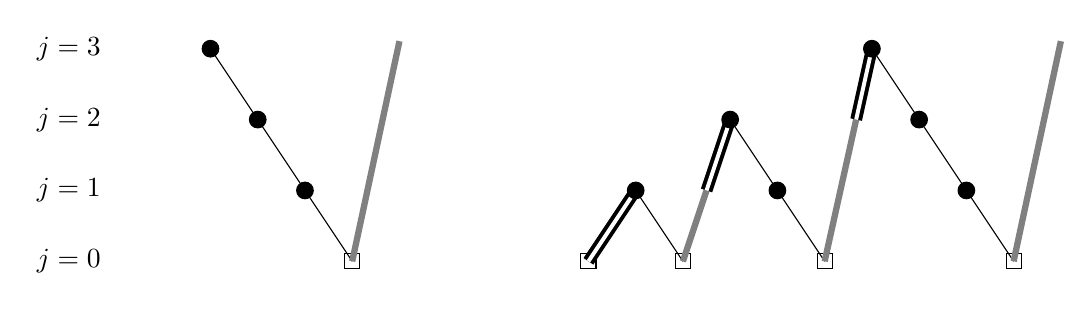
\begin{tikzpicture}[scale=1.2]
  \pgfmathsetmacro\hstep{0.5}
  \pgfmathsetmacro\vstep{0.75}
  \pgfmathsetmacro\ceps{0.08}   % size of square for coarse grid

% grid labels at left
  \node at (-6,3*\vstep) {$j=3$};
  \node at (-6,2*\vstep) {$j=2$};
  \node at (-6,\vstep) {$j=1$};
  \node at (-6,0.0) {$j=0$};

% 4-level slash-cycle
  \draw[black,thin] (-9*\hstep,3*\vstep) -- (-8*\hstep,2*\vstep) -- (-7*\hstep,\vstep) --  (-6*\hstep,0.0);
  \filldraw (-9*\hstep,3*\vstep) circle (2.5pt);
  \filldraw (-8*\hstep,2*\vstep) circle (2.5pt);
  \filldraw (-7*\hstep,\vstep) circle (2.5pt);
  \draw     (-6*\hstep-\ceps,-\ceps) rectangle (-6*\hstep+\ceps,+\ceps);
  \draw[gray,line width=0.8mm] (-6*\hstep,0.0) -- (-5*\hstep,3*\vstep+\ceps);

% coarse solve only
  \draw     (-\hstep-\ceps,-\ceps) rectangle (-\hstep+\ceps,+\ceps);
  \draw[black,double,line width=0.5mm,double distance=0.5mm] (-\hstep,0.0) -- (0.0,\vstep);
% 2-level slash-cycle
  \draw[black,thin] (0.0,\vstep) -- (\hstep,0.0);
  \filldraw (0.0,\vstep) circle (2.5pt);
  \draw     (\hstep-\ceps,-\ceps) rectangle (\hstep+\ceps,+\ceps);
  \draw[gray,line width=0.8mm] (\hstep,0.0) -- (1.5*\hstep,\vstep);
  \draw[black,double,line width=0.5mm,double distance=0.5mm] (1.5*\hstep,\vstep) -- (2*\hstep,2*\vstep);
% 3-level slash-cycle
  \draw[black,thin] (2*\hstep,2*\vstep) -- (3*\hstep,\vstep) --  (4*\hstep,0.0);
  \filldraw (2*\hstep,2*\vstep) circle (2.5pt);
  \filldraw (3*\hstep,\vstep) circle (2.5pt);
  \draw     (4*\hstep-\ceps,-\ceps) rectangle (4*\hstep+\ceps,+\ceps);
  \draw[gray,line width=0.8mm] (4*\hstep,0.0) -- (4.666667*\hstep,2*\vstep);
  \draw[black,double,line width=0.5mm,double distance=0.5mm] (4.666667*\hstep,2*\vstep) -- (5*\hstep,3*\vstep);
% 4-level slash-cycle
  \draw[black,thin] (5*\hstep,3*\vstep) -- (6*\hstep,2*\vstep) -- (7*\hstep,\vstep) --  (8*\hstep,0.0);
  \filldraw (5*\hstep,3*\vstep) circle (2.5pt);
  \filldraw (6*\hstep,2*\vstep) circle (2.5pt);
  \filldraw (7*\hstep,\vstep) circle (2.5pt);
  \draw     (8*\hstep-\ceps,-\ceps) rectangle (8*\hstep+\ceps,+\ceps);
  \draw[gray,line width=0.8mm] (8*\hstep,0.0) -- (9*\hstep,3*\vstep+\ceps);

\end{tikzpicture}

\caption{An F-cycle prepends shallower V-cycles, with a new prolongation $\hat P$ (double lines) generating initial iterates on finer levels.}
\label{fig:fcycle}
\end{figure}

Define \emph{solution prolongation} using canonical prolongation \eqref{eq:canonicalprolongation} and truncation:
\begin{equation}
\hat P w^{j-1} = \max\{P w^{j-1}, \varphi^{j}\}  \label{eq:solutionprolongation}
\end{equation}
After creating this initial iterate in $\mathcal{V}^j$ we do one or more V-cycles.  The following pseudocode implements this strategy.  Note there is no convergence criterion; the number of cycles is fixed.
\begin{pseudo*} \label{ps:mcdl-fcycle}
\pr{mcdl-fcycle}(J,F,\varphi,\id{nicycles}=1)\text{:} \\+
    $w^0=\varphi^0$ \qquad\qquad\qquad\qquad\qquad\quad \ct{admissible on the coarsest level} \\
    for $j=0,\dots,J$ \\+
        for $s=1,\dots,\id{nicycles}$ \qquad\qquad\qquad \ct{one or more V-cycles} \\+
            $\chi^j = \varphi^j - w^j$ \qquad\qquad\qquad\quad \ct{defect constraint on this level} \\
            $\ell^j[\cdot] := \ip{f}{\cdot}$ \\
            $F^j(y)[\cdot] := a(y,\cdot) - \ell^j[\cdot]$ \\
            $w^j \gets w^j+\pr{mcdl-vcycle}(j,F^j,\chi^j)$ \\-
        if $j < J$ \\+
            $w^j = \hat P w^{j-1}$ \qquad\qquad\qquad \ct{initial iterate for next level; see \eqref{eq:solutionprolongation}} \\--
    return $w^J$
\end{pseudo*}
Note that when \pr{mcdl-vcycle} is called on the coarsest level it reduces to the coarse solver, namely iterations of the smoother.

For PDEs one F-cycle often suffices to reach discretization error \cite{Trottenbergetal2001}.  However, because obstacle problem solutions have lower regularity, and because multilevel cycles are required to both remove low frequencies from the error \emph{and} find the discrete free boundary, we assume that in practice the F-cycle would generate an initial fine-level iterate for \pr{mcdl-solver}.

FIXME F-cycle results which only assess whether one F-cycle gets close to discretization error; in actual practice the performances is somewhat inconsistent, presumably because the nested iteration solution can be ``lucky'', or not so much, with respect to locating the free boundary on the next level; not a wonder drug, but a potentially-useful tool

Many variations on these V- and F-cycle strategies have not been tested in this section.  Most significantly, reference \cite{GraeserKornhuber2009} describe monotone, truncated, and Newton-based multigrid methods for obstacle problems which extend the MCD method.  These methods demonstrably improve performance for the classical problem when the coincidence set (active set) is geometrically complicated, but in various ways they require the implementation to keep track of the discrete active set.  There is also the older complementarity-problem multilevel method of \cite{BrandtCryer1983}, while \cite{Blumetal2004} proposes a ``cascadic'' multilevel approach with a conjugate-gradient smoother.


\section{Multigrid for the shallow-ice mass conservation problem} \label{sec:sia}

FIXME model problem in previous section has the wrong ``physics'' but correctly addresses the free boundary and obstacle nature of the glacier problem; glaciers as obstacle problems introduced by \cite{Calvoetal2002}; extended by \cite{Bueler2016,Bueler2020,JouvetBueler2012}, but these do not use multigrid; multigrid is applied to SIA in \cite{Jouvetetal2013,JouvetGraeser2013} with similar algorithm; we apply MCD because of its geometric clarity; there are other fast solution methods, for which theory is incomplete also, e.g.~PFAS in \cite{BrandtCryer1983} and inactive-set Newton-Multigrid \cite[Chapter 12]{Bueler2021}, and monotone and truncated multigrid \cite{GraeserKornhuber2009}

FIXME SIA model equations \cite{Bueler2016} with constants from \cite{Huybrechtsetal1996}; in this section we consider the steady-state problem; an 1D exact solution is Bueler profile from \cite{vanderVeen2013} section 5.3, Figure \ref{fig:siadatafigure}

\begin{figure}
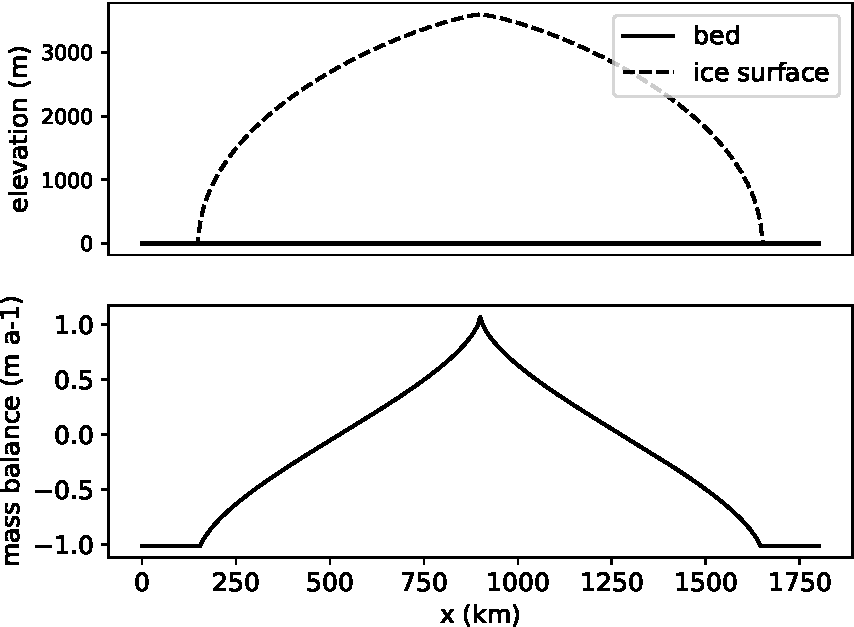
\includegraphics[width=0.7\textwidth]{fixfigs/siadatafigure.pdf}
\caption{\emph{Top:} Exact geometry solution for a flat-bed ice sheet.  \emph{Bottom:} Surface mass balance rate, the source term.}
\label{fig:siadatafigure}
\end{figure}

FIXME SIA modifications to smoother in 1D case

FIXME 1D results for smoother only

FIXME FAS version of MCD

FIXME for 2D domains use Firedrake


\section{Multigrid for Glen-Stokes glacier flow} \label{sec:stokes}

FIXME multigrid already used for Blatter-Pattyn model \cite{BrownSmithAhmadia2013}; for hybrid \cite{Jouvetetal2013,JouvetGraeser2013}; for Stokes \cite{IsaacStadlerGhattas2015} and \cite{Tuminaroetal2016} using AMG; one goal of this section is to make these approaches more understandable

FIXME obstacle problem view extended to Stokes by \cite{WirbelJarosch2020}

FIXME we use Schur complement \cite{Bueler2021,Elmanetal2014} and compare it to Vanka monolithic smoother \cite{Farrelletal2019}

FIXME time-dependent runs


\small

\bigskip
\bibliography{review}
\bibliographystyle{siam}

\normalsize

%\clearpage
\appendix

\section{Tables to assist the reader}

This review has been written attempting to use the simplest effective language and notation, but the new concepts are still substantial, and furthermore a number of different algorithms are discussed.  This Appendix may help the reader in managing the terminology, starting with acronyms in Table \ref{tab:acronyms} and notation in Table \ref{tab:notation}.  Tables \ref{tab:pseudocodespoisson} and \ref{tab:pseudocodesobstacle} list pseudocodes, for sections \ref{sec:subspace} and \ref{sec:obstacle} respectively, by page number.  All Tables are arranged alphabetically where possible.

\bigskip

\renewcommand{\arraystretch}{1.1}
\begin{longtable}{l|l}
\toprule
\textbf{Acronym} {\Large$\strut$} & \textbf{Definition} \\ \hline
FE & finite element \\
GMG & geometric multigrid \\
GS & Gauss-Seidel \\
MCD & multilevel constraint decomposition \\
MCDL & linear version of MCD \\
MSC & multilevel subspace corrections \\
PDE & partial differential equation \\
PGS & projected Gauss-Seidel \\
SIA & shallow ice approximation \\
VI & variational inequality \\
WU & work units \\ % final \\ required
\bottomrule
\caption{Acronyms.}
\label{tab:acronyms}
\end{longtable}

\renewcommand{\arraystretch}{1.2}
\begin{longtable}{l|l}
\toprule
\textbf{Symbol} {\Large$\strut$} & \textbf{Meaning} \\ \hline
$a(\cdot,\cdot)$ & bilinear form; for Poisson this is the left side of equation \eqref{eq:weakpoissonearly} \\
$\mathcal{D}^J$ & defect constraint set; $\mathcal{D}^J = \{v \ge \chi^J\}$ \\
$F(w)[\cdot]$ & residual of iterate $w$; $F(w)[v] = a(w,v) - \ip{f}{v}$ for Poisson \\
$F^j(w)[\cdot]$ & $j$th-level residual; $F^j(w)[v] = a(w,v) - \ell^j[v]$ for Poisson \\
$\mathcal{H}$ & Hilbert space for the continuum problem; $\mathcal{H}=H_0^1[0,1]$ for Poisson \\
$I(w)$ & scalar-valued objective function; $I(w) = \frac{1}{2} a(v,v) - \ip{f}{v}$ for Poisson \\
$J$ & level index of finest mesh \\
$j$ & index of mesh level; $j=0,1,\dots,J$ from coarse to fine \\
$\mathcal{K}$ & continuum constraint set; $\mathcal{K} = \{v \ge \varphi\} \subset \mathcal{H}$ \\
$\mathcal{K}^j$ & $j$th-level admissible functions; $\mathcal{K}^j = \{v \ge \phi^j\} \subset \mathcal{V}^j$ \\
$\ell[\cdot]$ & source linear functional, e.g.~$\ell[v] = \ip{f}{v}$ \\
$\ell^j[\cdot]$ & $j$th-level source; usually a restriction of the $j+1$ level residual \\
$m$ & number of degrees of freedom in discretized problem; $m=m_J$ \\
$m_j$ & number of nodes in $j$th-level; $\dim \mathcal{V}^j=m_j$ \\
$P$ & canonical prolongation of functions, $\mathcal{V}^{j-1} \to \mathcal{V}^j$; see Table \ref{tab:transfers} \\
$\hat P$ & solution prolongation of functions, $\mathcal{V}^{j-1} \to \mathcal{V}^j$; see Table \ref{tab:transfers} \\
$R$ & canonical restriction of linear functionals, $(\mathcal{V}^j)' \to (\mathcal{V}^{j-1})'$; see Table \ref{tab:transfers} \\
$\mR$ & monotone restriction of functions, $\mathcal{V}^j \to \mathcal{V}^{j-1}$; see Table \ref{tab:transfers} \\
$\mathcal{V}^h$ & finite element function space; $\mathcal{V}^h = \mathcal{V}^J$ \\
$\mathcal{V}^j$ & $j$th-level vector space \\
$(\mathcal{V}^j)'$ & dual space (linear functionals) of $\mathcal{V}^j$  \\
$x_p^j$ & $p$th node on $j$th-level mesh \\
$\varphi(x)$ & obstacle in continuum problem \\
$\varphi^j(x)$ & $j$th-level interpolant of continuum obstacle; \emph{not} equal to $\phi^j$ \\
$\phi^j(x)$ & $j$th-level obstacle; $\phi^j=\chi^j - \chi^{j-1}$ \\
$\chi^J(x)$ & fine-level defect obstacle; $\chi^J = \varphi^J - w^J$ for iterate $w^J$ \\
$\chi^j(x)$ & $j$th-level (monotone) restriction of defect obstacle; $\chi^{j-1} = \mR \chi^j$ \\
$\psi_p^j(x)$ & $j$th-level hat function at $x_p$ \\
$\ip{\cdot}{\cdot}$ & $L^2$ inner product \\
$\|\cdot\|$ & $L^2$ norm; $\|f\|=\ip{f}{f}^{1/2}$ \\
$\|\cdot\|_{\mathcal{H}}$ & norm on solution space; $\|f\|_{\mathcal{H}}^2 =\ip{f}{f} + \ip{f'}{f'}$ for $\mathcal{H}=H_0^1[0,1]$ \\  % final \\ required
\bottomrule
\caption{Notation for sections \ref{sec:subspace} and \ref{sec:obstacle}.}
\label{tab:notation}
\end{longtable}

\renewcommand{\arraystretch}{1.1}
\begin{longtable}{l|l|l}
\toprule
\textbf{Name} {\Large$\strut$} & \textbf{Page} & \textbf{Description} \\ \hline
\pr{euler-timestep} & \pageref{ps:euler-timestep} & forward Euler as a smoother iteration \\
\pr{gmg-coarsesolve} & \pageref{ps:gmg-coarsesolve} & geometric multigrid (GMG) coarse-level solver \\
\pr{gmg-vcycle} & \pageref{ps:gmg-vcycle} & efficiently-implementable GMG V-cycle \\
\pr{gs-sweep} & \pageref{ps:gs-sweep} & Gauss-Seidel (GS) iteration, a smoother \\
\pr{jacobi-sweep} & \pageref{ps:jacobi-sweep} & Jacobi iteration, a smoother \\
\pr{msc-downslash} & \pageref{ps:msc-downslash} & multilevel subspace corrections (MSC) slash-cycle, \\
  &  & \qquad V(1,0); calls a smoother \\
\pr{msc-solver} & \pageref{ps:msc-solver} & MSC solver; calls an MSC cycle \\
\pr{msc-vcycle} & \pageref{ps:msc-vcycle} & MSC V-cycle, V(1,1) \\
\pr{msc-upslash} & \pageref{ps:msc-upslash} & MSC slash-cycle, V(0,1) \\
\bottomrule
\caption{Pseudocodes for the Poisson equation (section \ref{sec:subspace}).}
\label{tab:pseudocodespoisson}
\end{longtable}

\begin{longtable}{l|l|l}
\toprule
\textbf{Name} {\Large$\strut$} & \textbf{Page} & \textbf{Description} \\ \hline
\pr{mcdl-fcycle} & \pageref{ps:mcdl-fcycle} & MCD F-cycle (nested iteration); calls \pr{mcdl-vcycle} \\
\pr{mcdl-vcycle} & \pageref{ps:mcdl-vcycle} & multilevel constraint decomposition (MCD) V-cycle \\
  &  & \qquad in linear case; calls \pr{p[gs$|$jacobi]-sweep} as smoother \\
\pr{mcdl-solver} & \pageref{ps:mcdl-solver} & MCD solver; calls \pr{mcdl-vcycle} \\
\pr{pgs} & \pageref{ps:pgs} & projected GS iteration, a smoother \\
\pr{pjacobi} & \pageref{ps:pjacobi} & projected Jacobi iteration, a smoother \\ % final \\ required
\bottomrule
\caption{Pseudocodes for the classical obstacle problem (section \ref{sec:obstacle}).}
\label{tab:pseudocodesobstacle}
\end{longtable}

\end{document}
